%%%%%%%%%%%%%%%%%%%%%%%%%%%%%%%%%%%%%%%%%%%%%%%%%%%%%%%%%%%%%%%%%%%%%%%%%
\documentclass[12pt,a4paper,final]{extreport}
\usepackage[utf8]{inputenc}
\usepackage{amsmath}
\usepackage{amsfonts}
\usepackage{amssymb}
\usepackage{bm}
\usepackage{array}
\usepackage{setspace}
\usepackage{verbatim}
\usepackage{adjustbox}
\usepackage{multirow}
\usepackage{caption}
\usepackage{subcaption}
\usepackage{ragged2e}
\justifying
\usepackage{tabularx}
\usepackage{booktabs}
\usepackage{float}
\usepackage{longtable}
\usepackage[table]{xcolor}
\renewcommand{\bibname}{References}
\usepackage[colorlinks]{hyperref}
\hypersetup{linkcolor={black},citecolor={black},urlcolor={black}}
\usepackage{graphicx}
\usepackage[left=3cm,right=2cm,top=3cm,bottom=3.5cm]{geometry}
\linespread{1.5}
\usepackage{titlesec}
\usepackage[yyyymmdd]{datetime}
\usepackage{fancyhdr}
\setlength{\headheight}{15pt}
\usepackage{algorithm}
\usepackage{algpseudocode}
\usepackage{enumitem}
\setlist{itemsep=2pt,topsep=4pt,parsep=0pt}
\usepackage{tikz}
\usetikzlibrary{arrows.meta,positioning,shapes.geometric,fit,calc,backgrounds}
\usepackage{pgfplots}
\pgfplotsset{compat=1.18}
\pgfplotsset{every axis/.append style={x tick label style={text height=1.6ex, text depth=0.35ex}}}

% --- Chart colours (validated categorical slots 1 and 2) ---
\definecolor{seriesA}{HTML}{2A78D6}   % baselines / series 1
\definecolor{seriesB}{HTML}{EB6834}   % proposed method / series 2
\definecolor{gridgray}{HTML}{D9D9D6}
\definecolor{seriesC}{HTML}{1BAF7A}   % series 3
\definecolor{seriesD}{HTML}{EDA100}   % series 4
\definecolor{inkgray}{HTML}{52514E}
% --- Diagram fills ---
\definecolor{boxblue}{HTML}{E3EEFB}
\definecolor{boxorange}{HTML}{FCE8DE}
\definecolor{boxgreen}{HTML}{DFF3EA}
\definecolor{boxgray}{HTML}{F1F1EF}
\definecolor{boxviolet}{HTML}{E9E6F7}

% --- Float placement: let text fill pages instead of leaving gaps ---
\renewcommand{\topfraction}{0.85}
\renewcommand{\bottomfraction}{0.7}
\renewcommand{\textfraction}{0.1}
\renewcommand{\floatpagefraction}{0.75}
\setcounter{topnumber}{3}
\setcounter{bottomnumber}{2}
\setcounter{totalnumber}{4}
\setlength{\textfloatsep}{14pt plus 4pt minus 4pt}
\setlength{\floatsep}{12pt plus 4pt minus 2pt}
\setlength{\intextsep}{12pt plus 4pt minus 2pt}
\captionsetup{font=small,labelfont=bf,skip=6pt}
\raggedbottom
\setlength{\emergencystretch}{2.5em}
\makeatletter
\renewcommand*\l@figure{\@dottedtocline{1}{1.5em}{3.3em}}
\makeatother

% --- Custom figure numbering format ---
\usepackage{chngcntr}          % allows linking counters
\counterwithin{figure}{section} % make figure numbering depend on section number
\renewcommand{\thefigure}{\thesection.\arabic{figure}} % custom figure numbering format

% Title/section formatting (matching sample)
\titleformat{\chapter}[display]
{\normalfont\rmfamily\huge\bfseries\color{black}}
{\chaptertitlename\ \thechapter}{20pt}{\huge}
\titleformat{\section}
{\normalfont\rmfamily\normalsize\bfseries\color{black}}
{\thesection}{16pt}{\large}
\titleformat{\subsection}
{\normalfont\rmfamily\small\bfseries\color{black}}
{\thesubsection}{16pt}{\normalsize}

\titlespacing{\chapter}{0pc}{0pc}{.5pc}
\titlespacing{\section}{0pc}{.8pc}{.2pc}
\titlespacing{\subsection}{0pc}{.8pc}{.1pc}

\thispagestyle{empty}
\begin{document}

% ================= TITLE PAGE =================
\begin{titlepage}
    \centering % Center all content on the page
    \pagenumbering{gobble} % Ensure no page number

    % --- Title and Subtitle ---
    {\Large\textbf{Neuromorphic Computing with Spiking Neural Networks: Efficient Deployment on Loihi 2 and TrueNorth}} \\
    \vspace*{0.3 cm}
    {\large\textbf{SEMINAR REPORT}} \\
    \vspace*{0.35cm}

    % --- Author Block ---
    {\emph{Submitted by}}\\[0.2cm]
    \textbf{Abhinav K R}\\
    \textbf{SNM23CA002}\\
    \textbf{to}\\
    \textbf{the APJ Abdul Kalam Technological University}\\
    \textbf{in partial fulfillment of the requirements for the award of the Degree of}\\
    \textbf{Bachelor of Technology}\\
    \textbf{in}\\
    \textbf{Computer Science and Engineering (Artificial Intelligence)}\\
    \vspace*{0.35cm}

    % --- Guidance Block ---
    {\textit{Under the guidance of}} \\[0.15cm]
    \textbf{Ms. Anu K A} \\
    \textbf{Assistant Professor} \\
    \textbf{Dept. of CSE} \\
    \vspace*{0.4cm}

    % --- Image ---
    
\includegraphics[scale=0.38]{snm.jpg} \\
    \vspace*{.4cm}

    % --- Department and College ---
    \textbf{Department of Computer Science and Engineering (Artificial Intelligence)} \\
    \textbf{SREE NARAYANA MANGALAM INSTITUTE OF}\\
    \textbf{MANAGEMENT AND TECHNOLOGY}\\
    \textbf{MALIANKARA}\\
    \vspace*{0.3cm}

    % --- Date ---
    October 2026

    \vfill
\end{titlepage}

% ================= CERTIFICATE =================
\clearpage
\thispagestyle{empty}
\begin{center}
{\fontsize{13}{16}\selectfont \textbf{DEPARTMENT OF COMPUTER SCIENCE \& ENGINEERING\\(ARTIFICIAL INTELLIGENCE)}}\\[10pt]
{\fontsize{13}{16}\selectfont \textbf{SREE NARAYANA MANGALAM INSTITUTE OF MANAGEMENT \&\\TECHNOLOGY, MALIANKARA}}\\[14pt]

\includegraphics[scale=0.32]{snm.jpg}\\[10pt]
\textbf{\Large CERTIFICATE}
\end{center}
\vspace{4pt}

\begingroup\setstretch{1.35}
\noindent\emph{This is to certify that the seminar report entitled {\bf{Neuromorphic Computing with Spiking Neural Networks: Efficient Deployment on Loihi 2 and TrueNorth}} submitted by {\bf Abhinav K R} ({\bf SNM23CA002}), to the {\bf Department of Computer Science and Engineering (Artificial Intelligence), SNM Institute of Management and Technology, Maliankara}, in partial fulfilment of the requirement for the award of B.Tech Degree in Computer Science and Engineering (Artificial Intelligence) is a bonafide record of the work carried out by the student.}\par
\endgroup

\vspace{1.8cm}

% Guide and HOD: each block is centred within its own half of the page
\noindent
\begin{minipage}[t]{0.48\textwidth}
\centering
\textbf{Guide}\\[28pt]
\textbf{Ms. Anu K A}\\
\textbf{Asst. Professor}\\
\textbf{Dept. of CSE}
\end{minipage}%
\hfill
\begin{minipage}[t]{0.48\textwidth}
\centering
\textbf{Head of the Department}\\[28pt]
\textbf{Ms. Lakshmi Anand}\\
\textbf{Asst. Professor}\\
\textbf{Dept. of CSE}
\end{minipage}

\vspace{1.1cm}

\noindent
\begin{minipage}[t]{\textwidth}
\centering
\textbf{Coordinator}\\[28pt]
\textbf{Ms. Surya T S}\\
\textbf{Asst. Professor}\\
\textbf{Dept. of CSE}
\end{minipage}

\newpage

% ================= DECLARATION =================
\thispagestyle{empty}
\begin{center}
\begin{huge}
\textbf{Declaration}
\end{huge}
\end{center}

\vskip0.5cm
I undersigned hereby declare that the seminar report \textbf{Neuromorphic Computing with Spiking Neural Networks: Efficient Deployment on Loihi 2 and TrueNorth}, submitted for partial fulfilment of the requirements for the award of degree of Bachelor of Technology of the APJ Abdul Kalam Technological University, Kerala is a bonafide work done by me under the supervision of \textbf{Ms. Anu K A}. This submission represents my ideas in my own words and where ideas or words of others have been included, I have adequately and accurately cited and referenced the original sources. I also declare that I have adhered to ethics of academic honesty and integrity and have not misrepresented or fabricated any data or idea or fact or source in my submission. I understand that any violation of the above will be a cause for disciplinary action by the institute and/or the University and can also evoke penal action from the sources which have thus not been properly cited or from whom proper permission has not been obtained. This report has not been previously formed the basis for the award of any degree, diploma or similar title of any other University.

\vspace{2cm}
\noindent
\begin{minipage}[t]{0.5\textwidth}
Place: Maliankara\\
Date: 22/10/2026
\end{minipage}%
\hfill
\begin{minipage}[t]{0.4\textwidth}
\centering
\textbf{Abhinav K R}\\
\textbf{SNM23CA002}
\end{minipage}

\newpage
\thispagestyle{plain}
\pagenumbering{Roman}
\setcounter{page}{1}
\addcontentsline{toc}{chapter}{Acknowledgement}
\begin{center}
\begin{huge}
\textbf{Acknowledgement}
\end{huge}
\end{center}
\vskip1cm
\hspace*{1 cm} Firstly, I thank God, the Almighty, with whose blessings, this seminar has been successfully completed.

I wish to give deep sense of acknowledgement to our Principal \textbf{Dr. Atmaram P}, for his constant encouragement and valuable advice throughout the course.

I am extremely grateful to \textbf{Ms. Lakshmi Anand}, Head of the Department of Computer Science and Engineering, for the valuable guidance through this humble endeavor. The highly enterprising attitude, patience for listening to my doubts, timely suggestions and guidance made my seminar a so-called reality in stipulated time.
I would also like to thank our seminar coordinator \textbf{Ms. Surya T S}, Assistant Professor, Department of Computer Science and Engineering and my seminar guide \textbf{Ms. Anu K A}, Assistant Professor, Department of Computer Science and Engineering for their gracious of encouragement and the valuable assistance.

I express my sincere gratitude to all the faculty members of the department of Computer Science and Engineering (Artificial Intelligence) for their co-operation and support to the seminar.

I also express my sincere gratitude to all my friends and my parents for their co-operation and constant inspiration.

\vspace{2cm}
\noindent\hfill
\begin{minipage}[t]{0.4\textwidth}
\centering
\textbf{Abhinav K R}
\end{minipage}

\newpage

% ================= ABSTRACT =================
\begin{center}
\begin{huge}
\textbf{Abstract}
\end{huge}
\end{center}

\addcontentsline{toc}{chapter}{Abstract}
\vskip0.3cm

\begingroup
\setstretch{1.15}
\paragraph{} Deep learning has achieved remarkable accuracy, but running it on conventional CPUs and GPUs consumes far more energy than real-time, battery-powered edge systems such as voice interfaces, autonomous vehicles, and surveillance drones can afford. Neuromorphic computing addresses this problem by imitating the brain: Spiking Neural Networks (SNNs) communicate through sparse, discrete events, and neuromorphic processors such as IBM's TrueNorth and Intel's Loihi 2 keep memory next to computation and perform work only when spikes arrive. This seminar presents a comparative study of four recent works that train, convert, and deploy SNNs on these two chips.

\paragraph{} Meszaros et al., the base paper, build a complete pipeline that trains SNNs with learnable synaptic delays using the event-based EventProp algorithm in mlGeNN and deploys them on Loihi 2 through the NetX format, improving feedforward keyword-spotting accuracy by up to 26.9 percentage points and running up to 18 times faster and with about 250 times less energy than an NVIDIA Jetson Orin Nano. Isik et al. implement five dataset-specific SNNs for multimodal sensor fusion in autonomous driving on Loihi-2, reporting a power efficiency of 103.94 GOP/s/W and sub-millisecond inference. Shrestha et al. map a Long Short-Term Memory network onto TrueNorth using discretised weights, piecewise-linear gates, burst-coded cell states, and a store-and-release synchronisation mechanism, consuming only 56 $\mu$J per sample. Brehove et al. convert standard quantised PyTorch networks into sigma-delta neural networks that exploit Loihi 2's graded spikes, achieving 16 times lower energy and about 40 times lower energy-delay product than an edge GPU and a real-time field deployment for drone detection.

\paragraph{} Comparing these approaches across training strategy, neural coding, hardware constraints, and measured efficiency reveals a consistent pattern: neuromorphic hardware delivers order-of-magnitude gains in energy and energy-delay product when the network's activity is sparse and its computation is mapped to the chip's native primitives---delays, graded spikes, or crossbar cores---while accuracy, latency, and input-output overheads remain the main trade-offs. The study concludes that pairing conventional deep-learning toolchains with hardware-aware conversion and event-based sensors is the most practical path to efficient neuromorphic deployment at the edge.

\vspace{0.5cm}
\noindent
\textbf{Keywords:} Neuromorphic Computing; Spiking Neural Networks; Intel Loihi 2; IBM TrueNorth; Synaptic Delays; EventProp; Sensor Fusion; Spike-Based LSTM; Sigma-Delta Neural Networks; ANN-to-SNN Conversion; Energy-Efficient Edge AI.
\endgroup

\newpage

% ================= TOC / LISTS =================
\thispagestyle{plain}
\begingroup
\setstretch{1.12}
\tableofcontents
\endgroup
\begingroup
\setstretch{1.2}
\listoffigures
\addcontentsline{toc}{chapter}{List of Figures}
\listoftables
\addcontentsline{toc}{chapter}{List of Tables}
\endgroup

% ================= LIST OF ABBREVIATIONS =================
\chapter*{List of Abbreviations}
\addcontentsline{toc}{chapter}{List of Abbreviations}

\begingroup
\setstretch{1.25}
\begin{longtable}{p{2.6cm}l}
\textbf{AER} & Address-Event Representation \\
\textbf{AI} & Artificial Intelligence \\
\textbf{AMP} & Accumulated Membrane Potential \\
\textbf{ANN} & Artificial Neural Network \\
\textbf{ASIC} & Application-Specific Integrated Circuit \\
\textbf{BPTT} & Backpropagation Through Time \\
\textbf{CAN} & Controller Area Network \\
\textbf{CPE} & Corelet Programming Environment \\
\textbf{CPU} & Central Processing Unit \\
\textbf{DL} & Deep Learning \\
\textbf{EDP} & Energy-Delay Product \\
\textbf{ERG} & Embedded Reber Grammar \\
\textbf{FP32} & 32-bit Floating Point \\
\textbf{FPGA} & Field-Programmable Gate Array \\
\textbf{FPS} & Frames Per Second \\
\textbf{GOP/s} & Giga-Operations per Second \\
\textbf{GPU} & Graphics Processing Unit \\
\textbf{GRU} & Gated Recurrent Unit \\
\textbf{HDF5} & Hierarchical Data Format version 5 \\
\textbf{IC} & Input Collection (module) \\
\textbf{IMU} & Inertial Measurement Unit \\
\textbf{INT8} & 8-bit Integer \\
\textbf{IO} & Input/Output \\
\textbf{IoT} & Internet of Things \\
\textbf{LIDAR} & Light Detection and Ranging \\
\textbf{LIF} & Leaky Integrate-and-Fire \\
\textbf{LSTM} & Long Short-Term Memory \\
\textbf{MAC} & Multiply-Accumulate \\
\textbf{mAP} & Mean Average Precision \\
\textbf{MSDD} & Multi-Sensor Drone Detection (dataset) \\
\textbf{MSE} & Mean Squared Error \\
\textbf{NetX} & Network Exchange (format) \\
\textbf{PL} & Phase Length \\
\textbf{RNN} & Recurrent Neural Network \\
\textbf{RPValue} & Represented Value \\
\textbf{S-LSTM} & Spike-Based Long Short-Term Memory \\
\textbf{SDNN} & Sigma-Delta Neural Network \\
\textbf{SHD} & Spiking Heidelberg Digits \\
\textbf{SLAYER} & Spike Layer Error Reassignment \\
\textbf{SNN} & Spiking Neural Network \\
\textbf{SoC} & System on Chip \\
\textbf{SRAM} & Static Random-Access Memory \\
\textbf{SSC} & Spiking Speech Commands \\
\textbf{SynOps} & Synaptic Operations \\
\textbf{YOLO} & You Only Look Once \\
\end{longtable}
\endgroup

\newpage

% ================= PAGE STYLE =================
\lhead{Neuromorphic Computing with SNNs on Loihi 2 and TrueNorth}
\chead{}
\rhead{}
\lfoot{\textit{Dept. of CSE (AI), SNMIMT}}
\cfoot{}
\rfoot{\thepage}
\renewcommand{\headrulewidth}{0.4pt}
\renewcommand{\footrulewidth}{0.4pt}
\pagestyle{fancy}
\fancypagestyle{plain}{%
  \fancyhf{}%
  \lfoot{\textit{Dept. of CSE (AI), SNMIMT}}%
  \rfoot{\thepage}%
  \renewcommand{\headrulewidth}{0pt}%
  \renewcommand{\footrulewidth}{0.4pt}}
\titleformat{\chapter}[display]
  {\normalfont\huge\bfseries\filcenter}
  {\chaptername\ \thechapter}{1ex}{\Huge}
\titlespacing*{\chapter}{0pt}{-10pt}{24pt}

\pagenumbering{arabic}
\setcounter{page}{1}


% ================= CHAPTER 1: INTRODUCTION =================
\chapter{Introduction}

\paragraph{} Deep neural networks now recognise speech, detect objects, and steer vehicles with remarkable accuracy, but they do so at a high energy cost. A conventional processor stores weights and activations in memory that is physically separate from its arithmetic units, so every layer of a network moves large amounts of data back and forth and performs dense multiply-accumulate (MAC) operations on every input, whether or not that input has changed. On a data-centre GPU this cost is tolerable; on a smart speaker, a car, or a drone running on a battery it is not \cite{p2,p4}. The human brain, by contrast, performs perception and control on about twenty watts, because its neurons communicate only through brief, sparse electrical pulses and store their state where they compute.

\paragraph{} \textbf{Neuromorphic computing} transfers these principles to silicon. \textbf{Spiking Neural Networks} (SNNs)---often called the third generation of neural network models---replace continuous activations with discrete events called \emph{spikes}, and neuromorphic processors execute them on many small cores that each hold the state of their own neurons and synapses. Computation is \emph{event-driven}: a neuron does work only when a spike arrives, and a core sends traffic only when one of its neurons fires. IBM's \textbf{TrueNorth} \cite{merolla2014} and Intel's \textbf{Loihi} \cite{davies2018} and \textbf{Loihi 2} \cite{orchard2021} are the best-known examples, and the works reviewed here report gains of one to three orders of magnitude in energy over CPUs and GPUs on suitable tasks \cite{p1,p2,p3,p4}.

\paragraph{} This seminar presents a comparative study of four works that deploy SNNs on these chips. Paper \cite{p1}, the base paper, by Meszaros et al., builds a \textbf{complete pipeline} that trains SNNs with learnable \textbf{synaptic delays} on GPUs and deploys them on Loihi 2 for keyword spotting. Paper \cite{p2}, by Isik et al., implements five SNNs for \textbf{multimodal sensor fusion} in autonomous driving on Loihi-2 and compares them with a CPU and a GPU. Paper \cite{p3}, by Shrestha et al., maps a \textbf{Long Short-Term Memory} (LSTM) network onto TrueNorth's spiking cores. Paper \cite{p4}, by Brehove et al., \textbf{converts} conventional quantised networks into \textbf{sigma-delta neural networks} that use Loihi 2's graded spikes, and deploys one in the field.

\section{General Background}

\paragraph{} Figure~\ref{fig:vonneumann} contrasts the two styles of computing. In the \textbf{von Neumann} architecture, a processor fetches weights and activations from shared memory over a bus, computes a dense layer, and writes the results back; the time and energy spent moving data---the \emph{memory wall}---dominate the cost of inference. A clock drives every unit at every cycle, and every input frame is processed completely even if it is almost identical to the previous one \cite{p4}. In a \textbf{neuromorphic} architecture, memory is distributed among many cores, each of which stores the synaptic weights and membrane states of its own neurons in local SRAM. Neurons integrate incoming spikes and fire only when their potential crosses a threshold, and spikes are routed between cores as small packets by a network-on-chip using \textbf{address-event representation} (AER) \cite{p3}. Energy is therefore spent roughly in proportion to spiking activity rather than to network size.

\begin{figure}[htbp]
\centering
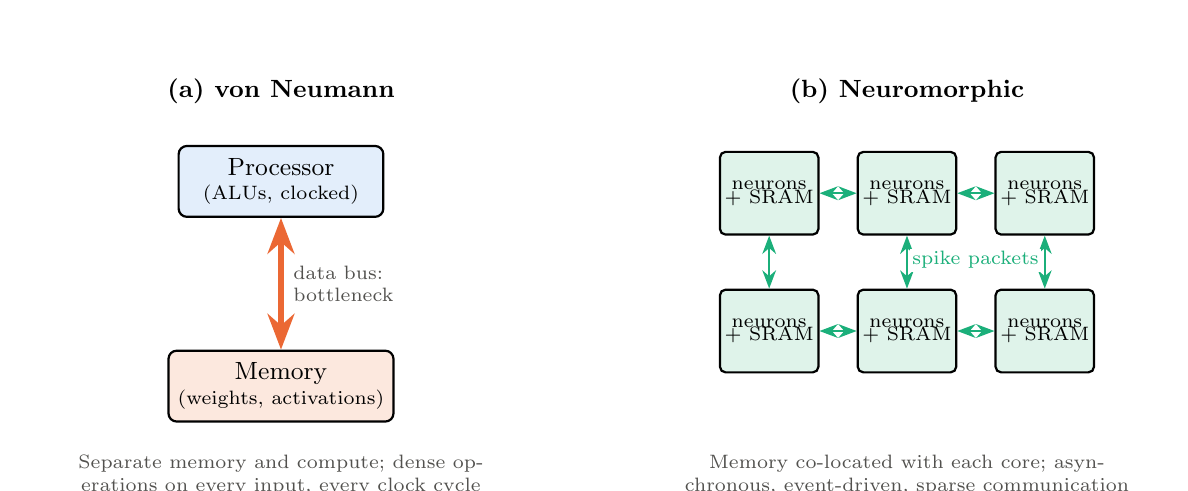
\begin{tikzpicture}[>=Stealth, thick,
  blk/.style={draw, rounded corners=3pt, minimum height=0.9cm, font=\small, align=center},
  core/.style={draw, rounded corners=2pt, fill=boxgreen, minimum width=1.25cm, minimum height=1.05cm, font=\scriptsize, align=center, inner sep=1pt},
  lab/.style={font=\small\bfseries},
  note/.style={font=\scriptsize, text=inkgray, align=center, text width=6.2cm}]
\node[blk, fill=boxblue, minimum width=2.6cm] (cpu) at (0,1.6) {Processor\\[-2pt]\scriptsize (ALUs, clocked)};
\node[blk, fill=boxorange, minimum width=2.6cm] (mem) at (0,-1.0) {Memory\\[-2pt]\scriptsize (weights, activations)};
\draw[<->, seriesB, line width=2.2pt] (cpu) -- node[right, font=\scriptsize, text=inkgray, align=left]{data bus:\\ bottleneck} (mem);
\node[lab] at (0,2.75) {(a) von Neumann};
\node[note, anchor=north] at (0,-1.75) {Separate memory and compute; dense operations on every input, every clock cycle};
\foreach \i in {0,1,2} \foreach \j in {0,1} {
  \node[core] (c\i\j) at (6.2+\i*1.75, 1.45-\j*1.75) {neurons\\[-3pt]+ SRAM};
}
\foreach \i/\k in {0/1,1/2} \foreach \j in {0,1} \draw[<->, seriesC] (c\i\j) -- (c\k\j);
\foreach \i in {0,1,2} \draw[<->, seriesC] (c\i0) -- (c\i1);
\node[font=\scriptsize, text=seriesC, fill=white, inner sep=1pt] at (8.82,0.6) {spike packets};
\node[lab] at (7.95,2.75) {(b) Neuromorphic};
\node[note, anchor=north] at (7.95,-1.75) {Memory co-located with each core; asynchronous, event-driven, sparse communication};
\end{tikzpicture}
\caption{Conventional von Neumann computing compared with event-driven neuromorphic computing}
\label{fig:vonneumann}
\end{figure}

\paragraph{} Two kinds of \textbf{sparsity} make this efficient. \emph{Spatial sparsity} means that at any moment only a small fraction of neurons are active, so most synapses do no work. \emph{Temporal sparsity} means that consecutive inputs---audio frames, video frames, sensor readings---change little, so a network that transmits only changes performs far fewer operations than one that recomputes everything \cite{p4}. Exploiting both requires suitable neuron models, suitable ways of encoding numbers in spikes, and training methods that respect the hardware's limited precision, connectivity, and memory. The four reviewed works approach these requirements from different directions: by learning richer \emph{temporal} computation through delays \cite{p1}, by applying SNNs to a demanding \emph{system-level} task \cite{p2}, by implementing a complex \emph{recurrent} architecture under severe hardware constraints \cite{p3}, and by \emph{converting} conventionally trained networks so that they exploit sparsity automatically \cite{p4}.

\section{Motivation}

\paragraph{} Three needs motivate this study. First, \textbf{edge intelligence}: keyword spotting, sensor fusion, and drone detection must run continuously on devices with tight power budgets, where cloud processing adds latency, depends on connectivity, and raises privacy concerns \cite{p1,p2}. Second, \textbf{latency}: autonomous driving and counter-drone systems need decisions within milliseconds, and batching inputs to make a GPU efficient conflicts with this requirement \cite{p1,p4}. Third, \textbf{programmability}: neuromorphic chips have been available to researchers for years, yet their adoption is limited because training SNNs is harder than training conventional networks and because each chip imposes its own constraints on weights, neurons, and connectivity \cite{p3,p4}. A clear picture of how recent works overcome these obstacles is therefore valuable.

\section{Problem Statement}

\paragraph{} \emph{Given a task that is naturally temporal or streaming---speech, multimodal sensor data, symbol sequences, or video---obtain a spiking neural network that achieves accuracy comparable to a conventional deep network, map it onto a neuromorphic processor within that processor's constraints on precision, connectivity, and neuron resources, and demonstrate lower energy, latency, or energy-delay product than conventional hardware.}

\section{Objectives}

\paragraph{} The objectives of this seminar are:
\begin{itemize}
  \item To introduce spiking neuron models, neural coding schemes, SNN training and conversion methods, and the TrueNorth and Loihi 2 architectures.
  \item To review in depth four works on SNN deployment for keyword spotting, sensor fusion, sequence learning, and video understanding.
  \item To compare their training strategies, coding schemes, hardware mappings, and measured efficiency.
  \item To identify open challenges and future research directions for practical neuromorphic edge computing.
\end{itemize}

\section{Scope}

\paragraph{} The seminar covers delay learning and deployment on Loihi 2 \cite{p1}, sensor fusion for autonomous driving on Loihi-2 \cite{p2}, spike-based recurrent networks on TrueNorth \cite{p3}, and ANN-to-SNN conversion with graded spikes on Loihi 2 \cite{p4}, together with the datasets, software frameworks, and metrics that these works use. Analogue and mixed-signal neuromorphic chips and on-chip learning are discussed only briefly.

\section{Advantages}

\paragraph{} Neuromorphic deployment of SNNs offers several advantages over conventional deep-learning hardware:
\begin{itemize}
  \item \textbf{Energy Efficiency:} work is done only when spikes occur, so sparse workloads consume a small fraction of GPU energy.
  \item \textbf{Low Latency:} inputs are processed as they arrive, without waiting to fill a batch.
  \item \textbf{Native Temporal Processing:} membrane dynamics and synaptic delays give networks built-in memory for time-varying signals.
  \item \textbf{Scalability:} chips tile into boards of many cores and chips that run larger networks without a shared memory bottleneck.
\end{itemize}

\section{Organization of the Report}

\paragraph{} \textbf{Chapter 2} introduces the theoretical foundations. \textbf{Chapter 3} reviews the four works in detail. \textbf{Chapter 4} compares the approaches, \textbf{Chapter 5} discusses applications, \textbf{Chapter 6} presents challenges and future directions, and \textbf{Chapter 7} concludes the report.

% ================= CHAPTER 2: THEORETICAL FOUNDATIONS =================
\chapter{Theoretical Foundations}

\paragraph{} This chapter introduces the concepts on which the reviewed works build: the principles of neuromorphic computing, spiking neuron models, ways of encoding numbers in spikes, methods for training and converting SNNs, synaptic delays, the TrueNorth and Loihi 2 processors and their software, and the metrics used to evaluate neuromorphic systems.

\section{Neuromorphic Computing Principles}

\paragraph{} Neuromorphic systems are built on three principles. The first is \textbf{event-driven computation}: instead of a global clock forcing every unit to compute at every cycle, a neuron updates its state when it receives a spike, and a spike is sent only when a neuron fires \cite{p3}. The second is \textbf{co-location of memory and compute}: each core keeps its neurons' weights and internal states in local SRAM, which avoids the costly transfers between processor and external memory that dominate conventional inference \cite{p4}. The third is \textbf{massive parallelism}: thousands of simple cores operate concurrently and exchange spikes asynchronously through a network-on-chip, so that larger networks are handled by adding cores or chips rather than by enlarging a single processor \cite{p2}.

\paragraph{} These principles make the energy of a neuromorphic computation roughly proportional to the number of \textbf{synaptic operations} (SynOps)---the number of spikes multiplied by their fan-out---rather than to the number of MACs in the equivalent dense network. The efficiency gain therefore depends on how sparse the network's activity is: a network that fires densely gains little, whereas one that fires rarely, or only when its input changes, can save one or more orders of magnitude \cite{p4}. Much of the work reviewed in Chapter~3 is about obtaining sparse activity without losing accuracy.

\section{Spiking Neuron Models}

\paragraph{} The most widely used neuron model in neuromorphic hardware is the \textbf{Leaky Integrate-and-Fire} (LIF) neuron, used directly in \cite{p1} and in variant forms on both chips. Its membrane potential $V(t)$ integrates an input current $I(t)$ while leaking towards a resting value:
\begin{equation}
\tau_m\frac{dV}{dt}=-\big(V-V_{\mathrm{rest}}\big)+R\,I(t),
\end{equation}
where $\tau_m$ is the membrane time constant and $R$ the membrane resistance. When $V$ reaches a threshold $\vartheta$, the neuron emits a spike and $V$ is reset to $V_{\mathrm{reset}}$. In discrete time, as executed on chip, the update for neuron $j$ becomes
\begin{equation}
V_j[t]=\alpha\,V_j[t-1]+\sum_{i}w_{ij}\,s_i[t],\qquad s_j[t]=\begin{cases}1, & V_j[t]\ge\vartheta\\ 0, & \text{otherwise}\end{cases}
\end{equation}
with decay factor $\alpha=e^{-\Delta t/\tau_m}$, synaptic weights $w_{ij}$, and binary input spikes $s_i[t]\in\{0,1\}$. With \textbf{exponential synapses}, each input spike instead adds to a synaptic current that itself decays with time constant $\tau_s$, smoothing the input \cite{p1}. Figure~\ref{fig:lif} shows the resulting behaviour: a weak input charges the membrane without reaching threshold and the potential leaks away when the input stops, whereas a stronger input drives the neuron to fire regularly, with a rate that increases with input strength.

\begin{figure}[htbp]
\centering
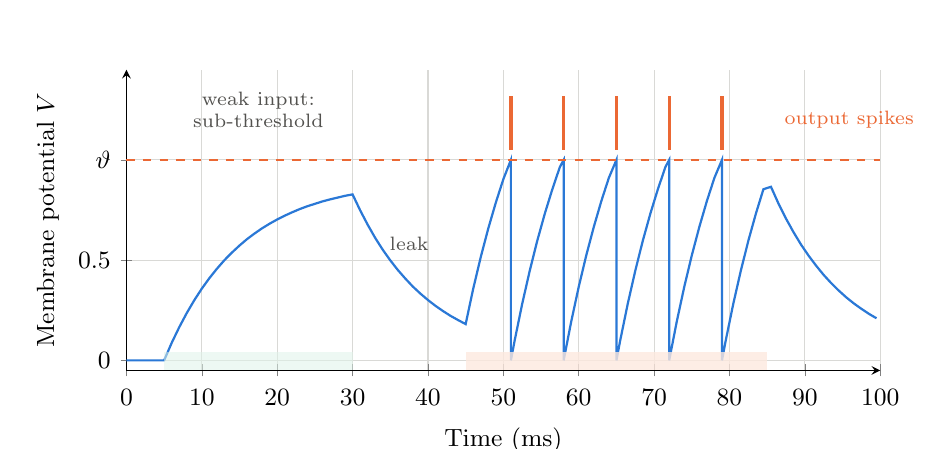
\begin{tikzpicture}
\begin{axis}[width=0.92\textwidth, height=5.4cm, xmin=0, xmax=100, ymin=-0.05, ymax=1.45,
  xlabel={Time (ms)}, ylabel={Membrane potential $V$}, ytick={0,0.5,1}, yticklabels={0,0.5,$\vartheta$},
  axis lines=left, grid=major, grid style={gridgray}, tick label style={font=\small}, label style={font=\small},
  clip=false]
\addplot[seriesA, thick] coordinates {(0,0.000) (5,0.000) (6,0.087) (7,0.165) (8,0.236) (9,0.300) (10,0.358) (11,0.410) (12,0.457) (13,0.500) (14,0.538) (15,0.573) (16,0.605) (17,0.633) (18,0.659) (19,0.682) (20,0.703) (21,0.722) (22,0.739) (23,0.755) (24,0.769) (25,0.781) (26,0.793) (27,0.803) (28,0.812) (29,0.821) (30,0.828) (31,0.749) (32,0.677) (33,0.611) (34,0.552) (35,0.499) (36,0.451) (37,0.408) (38,0.368) (39,0.333) (40,0.301) (41,0.272) (42,0.246) (43,0.222) (44,0.201) (45,0.181) (46,0.357) (47,0.515) (48,0.658) (49,0.787) (50,0.904) (51,1.000) (51,0.000) (51,0.000) (51.5,0.099) (52.5,0.282) (53.5,0.447) (54.5,0.597) (55.5,0.732) (56.5,0.854) (57.5,0.965) (58,1.000) (58,0.000) (58,0.000) (59,0.193) (60,0.367) (61,0.524) (62,0.666) (63,0.795) (64,0.911) (65,1.000) (65,0.000) (65,0.000) (65.5,0.099) (66.5,0.282) (67.5,0.447) (68.5,0.597) (69.5,0.732) (70.5,0.854) (71.5,0.965) (72,1.000) (72,0.000) (72,0.000) (73,0.193) (74,0.367) (75,0.524) (76,0.666) (77,0.795) (78,0.911) (79,1.000) (79,0.000) (79,0.000) (79.5,0.099) (80.5,0.282) (81.5,0.447) (82.5,0.597) (83.5,0.732) (84.5,0.854) (85.5,0.866) (86.5,0.782) (87.5,0.707) (88.5,0.639) (89.5,0.577) (90.5,0.522) (91.5,0.472) (92.5,0.426) (93.5,0.385) (94.5,0.348) (95.5,0.314) (96.5,0.284) (97.5,0.257) (98.5,0.232) (99.5,0.210)};
\draw[seriesB, dashed, thick] (axis cs:0,1) -- (axis cs:100,1);
\pgfplotsinvokeforeach{51.0,58.0,65.0,72.0,79.0}{ \draw[seriesB, very thick] (axis cs:#1,1.05) -- (axis cs:#1,1.32); }
\fill[boxgreen, opacity=0.55] (axis cs:5,-0.05) rectangle (axis cs:30,0.04);
\fill[boxorange, opacity=0.8] (axis cs:45,-0.05) rectangle (axis cs:85,0.04);
\node[font=\scriptsize, text=inkgray, align=center] at (axis cs:17.5,1.25) {weak input:\\ sub-threshold};
\node[font=\scriptsize, text=inkgray] at (axis cs:37.5,0.58) {leak};
\node[font=\scriptsize, text=seriesB, anchor=west] at (axis cs:86,1.2) {output spikes};
\end{axis}
\end{tikzpicture}
\caption{Simulated leaky integrate-and-fire neuron: a weak input (green) stays below threshold and leaks away, while a stronger input (orange) produces regular output spikes}
\label{fig:lif}
\end{figure}

\paragraph{} Other neuron models are also used. TrueNorth neurons are configurable integrate-and-fire units with linear leak, stochastic thresholds, and saturating negative thresholds, which \cite{p3} exploits to build store-and-release circuits. Loihi 2 neurons are \textbf{programmable}: a small microcode program defines how the neuron updates its state, so new models such as the sigma-delta neuron of \cite{p4} can be implemented without changing the hardware. Output layers are often \textbf{non-firing leaky integrators} whose potentials are read out directly; in \cite{p1} the class decision is the output neuron with the largest exponentially weighted integral of its voltage over the sample.

\section{Neural Coding Schemes}

\paragraph{} Because spikes are all-or-nothing events, numerical values must be \emph{encoded} in their timing or number. Figure~\ref{fig:coding} illustrates the four schemes that appear in the reviewed works. In \textbf{rate coding}, a value is represented by the number of spikes in a window, often generated stochastically; it is robust but needs long windows for high precision \cite{p3}. In \textbf{burst coding}, the value is the number of spikes emitted in a consecutive burst, which correlates more tightly with the represented value than random rate codes and is used in \cite{p3} for the LSTM cell state. In \textbf{temporal coding}, information lies in precise spike times, which delays exploit \cite{p1}. Finally, Loihi 2 supports \textbf{graded spikes} that carry an integer payload; in \textbf{sigma-delta coding} a neuron sends a graded spike containing the \emph{change} in its activation only when that change exceeds a threshold, so a static input produces no traffic at all \cite{oconnor2016,p4}.

\begin{figure}[htbp]
\centering
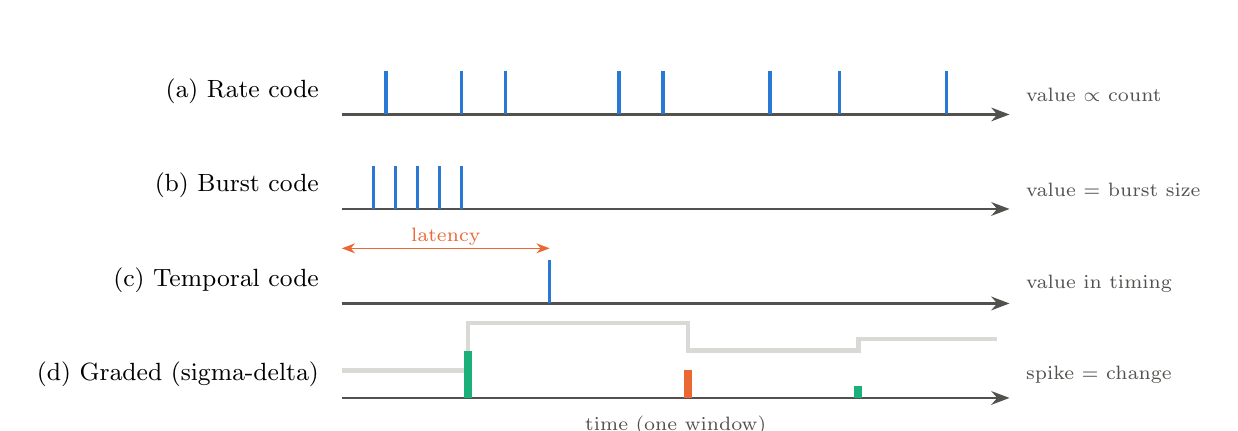
\begin{tikzpicture}[>=Stealth, thick, xscale=0.8, spk/.style={seriesA, line width=1.3pt}]
\foreach \y/\t in {3.6/{(a) Rate code},2.4/{(b) Burst code},1.2/{(c) Temporal code},0/{(d) Graded (sigma-delta)}} {
  \node[font=\small, anchor=east] at (-0.2,\y+0.3) {\t};
  \draw[->, inkgray] (0,\y) -- (10.6,\y);
}
\foreach \x in {0.7,1.9,2.6,4.4,5.1,6.8,7.9,9.6} \draw[spk] (\x,3.6) -- (\x,4.15);
\node[font=\scriptsize, text=inkgray, anchor=west] at (10.7,3.85) {value $\propto$ count};
\foreach \x in {0.5,0.85,1.2,1.55,1.9} \draw[spk] (\x,2.4) -- (\x,2.95);
\node[font=\scriptsize, text=inkgray, anchor=west] at (10.7,2.65) {value = burst size};
\draw[spk] (3.3,1.2) -- (3.3,1.75);
\draw[<->, seriesB, thin] (0,1.9) -- node[above, font=\scriptsize, text=seriesB, inner sep=1pt]{latency} (3.3,1.9);
\node[font=\scriptsize, text=inkgray, anchor=west] at (10.7,1.45) {value in timing};
\draw[gridgray, line width=1.6pt] (0,0.35) -- (2.0,0.35) -- (2.0,0.95) -- (5.5,0.95) -- (5.5,0.6) -- (8.2,0.6) -- (8.2,0.75) -- (10.4,0.75);
\draw[seriesC, line width=3pt] (2.0,0) -- (2.0,0.6);
\draw[seriesB, line width=3pt] (5.5,0) -- (5.5,0.35);
\draw[seriesC, line width=3pt] (8.2,0) -- (8.2,0.15);
\node[font=\scriptsize, text=inkgray, anchor=west] at (10.7,0.3) {spike = change};
\node[font=\scriptsize, text=inkgray] at (5.3,-0.35) {time (one window)};
\end{tikzpicture}
\caption{Neural coding schemes used in the reviewed works: rate and burst codes on TrueNorth \cite{p3}, spike timing exploited by delays \cite{p1}, and graded sigma-delta spikes on Loihi 2 \cite{p4}; in (d) the grey line is the activation and bar heights are spike payloads}
\label{fig:coding}
\end{figure}

\section{Training Spiking Neural Networks}

\paragraph{} The spike function is a step, so its derivative is zero almost everywhere and standard backpropagation cannot be applied directly. Two families of methods address this. \textbf{Direct training} treats the SNN as a recurrent network unrolled in time and trains it with \textbf{Backpropagation Through Time} (BPTT). \emph{Surrogate-gradient} methods replace the spike derivative with a smooth function; \textbf{SLAYER} \cite{shrestha2018}, part of Intel's Lava-DL library, assigns errors back through time in this way and is used to train sigma-delta networks for Loihi 2. These methods must store the whole time series of every neuron, which makes training memory-hungry and slow \cite{p4}. \textbf{EventProp} \cite{wunderlich2021} instead computes \emph{exact} gradients with an adjoint system that runs backwards in time and needs to store neuron states only at spike times. Because its backward pass has the same event-driven structure as the forward pass, it can be implemented efficiently on GPUs in the mlGeNN library and extended to learn synaptic delays \cite{p1}.

\paragraph{} \textbf{ANN-to-SNN conversion} sidesteps spike gradients: a conventional network is trained with standard tools and then translated into an SNN. Classic conversion represents each ReLU activation by a spike rate, which needs many timesteps per input for accurate rates. Paper \cite{p4} instead converts a quantised network into a sigma-delta network whose graded spikes carry exact integer changes, while \cite{p3} trains a conventional LSTM under hardware-motivated constraints and then approximates it with spiking circuits.

\section{Synaptic Delays}

\paragraph{} In biological networks, spikes take different amounts of time to travel along different axons, and these \textbf{synaptic delays} contribute to learning and to detecting coincident inputs \cite{p1}. Adding a delay $d_{ij}$ to each connection changes the input to neuron $j$ to
\begin{equation}
I_j(t)=\sum_{i}w_{ij}\,s_i\big(t-d_{ij}\big),
\end{equation}
so a neuron can respond to a particular \emph{temporal pattern} of input spikes rather than only to their total. Figure~\ref{fig:delays} shows the idea: three inputs that fire at different times reach the target simultaneously because each connection has a different delay, and the coincident arrival drives the neuron above threshold. Networks with learnable delays can compute a richer class of functions than networks with learnable weights alone, and they achieve state-of-the-art results in keyword recognition \cite{p1}. Loihi 2 supports synaptic delays of up to 62 timesteps in hardware.

\begin{figure}[htbp]
\centering
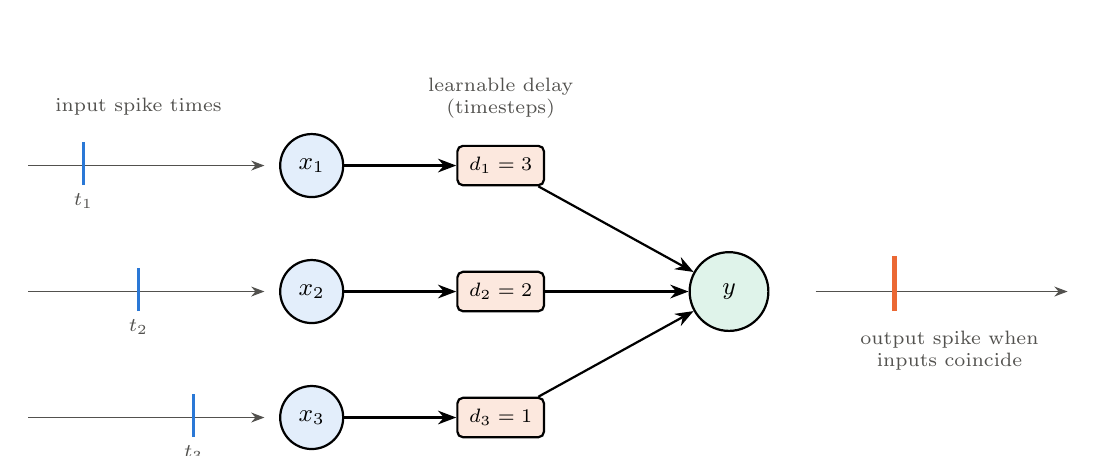
\begin{tikzpicture}[>=Stealth, thick,
  nrn/.style={draw, circle, fill=boxblue, minimum size=0.8cm, font=\small, inner sep=0pt},
  dl/.style={draw, rounded corners=2pt, fill=boxorange, font=\scriptsize, minimum width=1.1cm, minimum height=0.5cm}]
\foreach \y/\n/\t/\d in {1.6/1/1/3,0/2/2/2,-1.6/3/3/1} {
  \node[nrn] (n\n) at (0,\y) {$x_{\n}$};
  \draw[->, inkgray, thin] (-3.6,\y) -- (-0.6,\y);
  \draw[seriesA, line width=1.3pt] (-3.6+\t*0.7,\y-0.25) -- (-3.6+\t*0.7,\y+0.3);
  \node[font=\scriptsize, text=inkgray] at (-3.6+\t*0.7,\y-0.45) {$t_{\n}$};
  \node[dl] (d\n) at (2.4,\y) {$d_{\n}=\d$};
  \draw[->] (n\n) -- (d\n);
}
\node[nrn, fill=boxgreen, minimum size=1.0cm] (out) at (5.3,0) {$y$};
\foreach \n in {1,2,3} \draw[->] (d\n) -- (out);
\draw[->, inkgray, thin] (6.4,0) -- (9.6,0);
\draw[seriesB, line width=1.6pt] (7.4,-0.25) -- (7.4,0.45);
\node[font=\scriptsize, text=inkgray, align=center] at (8.1,-0.75) {output spike when\\ inputs coincide};
\node[font=\scriptsize, text=inkgray] at (-2.2,2.35) {input spike times};
\node[font=\scriptsize, text=inkgray, align=center] at (2.4,2.45) {learnable delay\\ (timesteps)};
\end{tikzpicture}
\caption{Coincidence detection with synaptic delays: inputs that fire at $t_1<t_2<t_3$ arrive together because the earliest input has the longest delay}
\label{fig:delays}
\end{figure}

\section{Neuromorphic Hardware Platforms}

\paragraph{} \textbf{IBM TrueNorth} \cite{merolla2014} consists of 4096 neurosynaptic cores, each with 256 input axons, 256 neurons, and a $256\times256$ crossbar of programmable binary synapses, giving one million neurons and 268 million synapses. Each neuron can use at most four different synaptic weight values, selected by the type of the input axon, and weights are 9-bit signed integers. The chip normally advances in 1 ms \emph{ticks}, within which membrane potentials are updated and spikes are routed asynchronously; a spike can target any single axon on the chip, and active power is proportional to firing activity \cite{p3}. Networks are described as \textbf{corelets}---reusable blocks of cores with defined inputs and outputs---in the object-oriented Corelet Programming Environment.

\paragraph{} \textbf{Intel Loihi 2} \cite{orchard2021}, the successor of Loihi \cite{davies2018}, is a fully asynchronous chip fabricated on the Intel~4 process. It contains 120 neuromorphic cores, each supporting about 8k neurons whose weights and states are held in local SRAM, together with six embedded processor cores and a 10~Gbps Ethernet spike interface \cite{p1,p4}. Its key features for the reviewed works are \textbf{programmable microcode neurons}, \textbf{graded spikes} with integer payloads of up to 16 bits, and \textbf{synaptic delays} of up to 62 timesteps. Chips are deployed on the single-chip Oheo Gulch board, the 8-chip Kapoho Point board---which, according to \cite{p2}, provides 1024 cores and 8.4 million neurons---and a 16-chip VPX board \cite{p4}. Figure~\ref{fig:loihi2} sketches the chip, and Table~\ref{tab:hw} compares the two processors.

\begin{figure}[htbp]
\centering
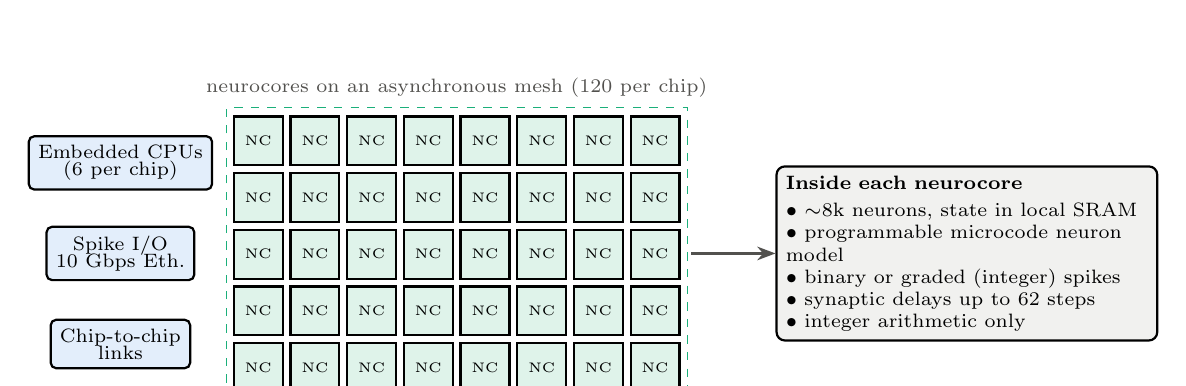
\begin{tikzpicture}[>=Stealth, thick,
  nc/.style={draw, fill=boxgreen, minimum size=0.62cm, inner sep=0pt, font=\tiny},
  side/.style={draw, rounded corners=2pt, fill=boxblue, minimum width=1.6cm, minimum height=0.55cm, font=\scriptsize, align=center},
  callout/.style={draw, rounded corners=3pt, fill=boxgray, font=\scriptsize, align=left, text width=4.6cm}]
\foreach \i in {0,...,7} \foreach \j in {0,...,4} \node[nc] at (\i*0.72,\j*0.72) {NC};
\draw[seriesC, dashed, thin] (-0.4,-0.4) rectangle (5.45,3.3);
\node[font=\scriptsize, text=inkgray] at (2.52,3.55) {neurocores on an asynchronous mesh (120 per chip)};
\foreach \j/\t in {2.6/{Embedded CPUs\\[-2pt](6 per chip)},1.45/{Spike I/O\\[-2pt]10 Gbps Eth.},0.3/{Chip-to-chip\\[-2pt]links}} \node[side] at (-1.75,\j) {\t};
\node[callout] (co) at (9.0,1.45) {\textbf{Inside each neurocore}\\[2pt]
$\bullet$ $\sim$8k neurons, state in local SRAM\\
$\bullet$ programmable microcode neuron model\\
$\bullet$ binary or graded (integer) spikes\\
$\bullet$ synaptic delays up to 62 steps\\
$\bullet$ integer arithmetic only};
\draw[->, inkgray] (5.5,1.45) -- (co.west);
\end{tikzpicture}
\caption{Simplified view of a Loihi 2 chip, based on the descriptions in \cite{p1,p4}}
\label{fig:loihi2}
\end{figure}

{\renewcommand{\arraystretch}{1.12}
\begin{table}[htbp]
\centering
\caption{Comparison of the neuromorphic processors used in the reviewed works}\label{tab:hw}
\small
\begin{tabularx}{\textwidth}{|p{3.0cm}|X|X|}
\hline
\textbf{Feature} & \textbf{IBM TrueNorth \cite{p3,merolla2014}} & \textbf{Intel Loihi 2 \cite{p1,p2,p4}} \\ \hline
Cores per chip & 4096 & 120 (128 reported in \cite{p2}) \\ \hline
Neurons & 256 per core; 1 million per chip & $\sim$8k per core \\ \hline
Synapses & $256\times256$ binary crossbar per core; 268 million & Configurable; weights in local SRAM \\ \hline
Weight precision & 9-bit signed; at most 4 values per neuron & Integer; 8-bit weights in \cite{p1,p4} \\ \hline
Spikes & Binary & Binary or graded (integer payload) \\ \hline
Neuron model & Fixed, configurable integrate-and-fire & Programmable microcode \\ \hline
Delays & Configurable axonal delays & Up to 62 timesteps \\ \hline
Time base & 1 ms ticks (faster than real time possible) & Algorithmic timesteps, asynchronous \\ \hline
Programming & Corelet Programming Environment & Lava, Lava-DL, NetX, NxKernel \\ \hline
\end{tabularx}
\end{table}}

\section{Software Frameworks}

\paragraph{} Software determines how easily a network reaches the chip. For Loihi 2, Intel's open-source \textbf{Lava} framework provides processes and a runtime, and \textbf{Lava-DL} adds SLAYER training, a rate-based \emph{Bootstrap} method, and \textbf{NetX}, an HDF5-based format for importing trained models \cite{p2}. \textbf{NxKernel}, available to members of the Intel Neuromorphic Research Community, maps networks to cores efficiently and provides power and timing probes \cite{p1,p4}. \textbf{mlGeNN}, built on the GPU-optimised GeNN simulator, supports EventProp training and exports to NetX \cite{p1}. TrueNorth networks are composed as corelets in the \textbf{Corelet Programming Environment} \cite{p3}, and \cite{p4} shows that standard \textbf{PyTorch} training and quantisation can be the front end of a neuromorphic pipeline.

\section{Evaluation Metrics}

\paragraph{} Neuromorphic systems are judged on task quality and on efficiency, and the reviewed works use several metrics (Table~\ref{tab:metrics}). Task quality is measured by \textbf{classification accuracy}, \textbf{mean average precision} (mAP) for detection, and \textbf{mean squared error} (MSE) for regression. Efficiency is measured by \textbf{energy per inference}, split into \emph{static} energy, consumed whenever the chip is powered, and \emph{dynamic} energy, caused by computation; by \textbf{latency} from input to output; by \textbf{throughput} in frames or operations per second; and by \textbf{power efficiency} in operations per second per watt. Because designs can trade speed for energy, the \textbf{energy-delay product} (EDP),
\begin{equation}
\mathrm{EDP}=E_{\mathrm{inference}}\times T_{\mathrm{latency}},
\end{equation}
summarises both, with lower values being better \cite{p1,p4}. Finally, \textbf{sparsity} is measured as the ratio of synaptic operations on the chip to the MACs of the equivalent ANN \cite{p4}.

{\renewcommand{\arraystretch}{1.15}
\begin{table}[htbp]
\centering
\caption{Evaluation metrics used in the reviewed works}\label{tab:metrics}
\small
\begin{tabularx}{\textwidth}{|p{3.6cm}|X|p{2.4cm}|}
\hline
\textbf{Metric} & \textbf{Meaning} & \textbf{Used in} \\ \hline
Accuracy, mAP, MSE & Task quality (classification, detection, regression) & \cite{p1,p3,p4} \\ \hline
Energy per inference & Total, static, and dynamic energy per sample or frame & \cite{p1,p3,p4} \\ \hline
Latency & Time from input to corresponding output & \cite{p1,p2,p3,p4} \\ \hline
Throughput & Frames per second or GOP/s & \cite{p2,p4} \\ \hline
Power efficiency & GOP/s/W or pJ per operation & \cite{p2} \\ \hline
Energy-delay product & Energy $\times$ latency (lower is better) & \cite{p1,p4} \\ \hline
Sparsity, resources & SynOps ratio, cores used, neuron density & \cite{p3,p4} \\ \hline
\end{tabularx}
\end{table}}

\section{Taxonomy of Approaches}

\paragraph{} Figure~\ref{fig:taxonomy} organises the reviewed works along four dimensions: how the spiking network is obtained, how information is coded, which hardware it targets, and which application it serves. The works are complementary: \cite{p1} and \cite{p4} represent the two main training routes---direct event-based training and conversion---while \cite{p3} shows how a complex recurrent architecture can be built from spiking circuits, and \cite{p2} studies the system-level benefit of neuromorphic hardware for a demanding application.

\begin{figure}[htbp]
\centering
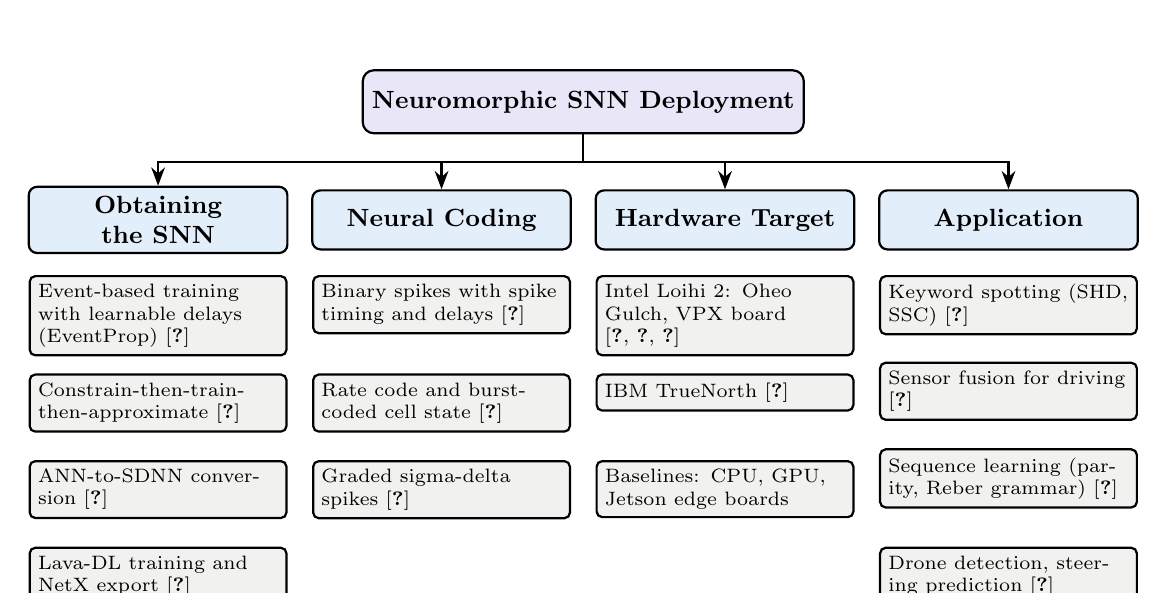
\begin{tikzpicture}[>=Stealth, thick,
  root/.style={draw, rounded corners=4pt, fill=boxviolet, font=\small\bfseries, minimum width=5.6cm, minimum height=0.8cm, align=center},
  cat/.style={draw, rounded corners=3pt, fill=boxblue, font=\small\bfseries, text width=3.05cm, align=center, minimum height=0.75cm},
  leaf/.style={draw, rounded corners=2pt, fill=boxgray, font=\scriptsize, text width=3.05cm, align=left, inner sep=3pt}]
\node[root] (r) at (5.4,0) {Neuromorphic SNN Deployment};
\foreach \x/\n/\t in {0/a/Obtaining the SNN,3.6/b/Neural Coding,7.2/c/Hardware Target,10.8/d/Application} {
  \node[cat] (\n) at (\x,-1.5) {\t};
  \draw[->] (r.south) -- ++(0,-0.35) -| (\n.north);
}
\node[leaf, anchor=north] (a1) at (0,-2.2) {Event-based training with learnable delays (EventProp) \cite{p1}};
\node[leaf, anchor=north] (a2) at (0,-3.45) {Constrain-then-train-then-approximate \cite{p3}};
\node[leaf, anchor=north] (a3) at (0,-4.55) {ANN-to-SDNN conversion \cite{p4}};
\node[leaf, anchor=north] (a4) at (0,-5.65) {Lava-DL training and NetX export \cite{p2}};
\node[leaf, anchor=north] (b1) at (3.6,-2.2) {Binary spikes with spike timing and delays \cite{p1}};
\node[leaf, anchor=north] (b2) at (3.6,-3.45) {Rate code and burst-coded cell state \cite{p3}};
\node[leaf, anchor=north] (b3) at (3.6,-4.55) {Graded sigma-delta spikes \cite{p4}};
\node[leaf, anchor=north] (c1) at (7.2,-2.2) {Intel Loihi 2: Oheo Gulch, VPX board \cite{p1,p2,p4}};
\node[leaf, anchor=north] (c2) at (7.2,-3.45) {IBM TrueNorth \cite{p3}};
\node[leaf, anchor=north] (c3) at (7.2,-4.55) {Baselines: CPU, GPU, Jetson edge boards};
\node[leaf, anchor=north] (d1) at (10.8,-2.2) {Keyword spotting (SHD, SSC) \cite{p1}};
\node[leaf, anchor=north] (d2) at (10.8,-3.3) {Sensor fusion for driving \cite{p2}};
\node[leaf, anchor=north] (d3) at (10.8,-4.4) {Sequence learning (parity, Reber grammar) \cite{p3}};
\node[leaf, anchor=north] (d4) at (10.8,-5.65) {Drone detection, steering prediction \cite{p4}};
\end{tikzpicture}
\caption{Taxonomy of the neuromorphic SNN deployment approaches reviewed in this seminar}
\label{fig:taxonomy}
\end{figure}

\section{Chapter Summary}

\paragraph{} SNNs compute with sparse events, and neuromorphic processors turn this sparsity into energy savings. Obtaining accurate SNNs requires direct training or conversion, and each choice interacts with the hardware: TrueNorth offers many simple, tightly constrained cores, while Loihi 2 offers programmable neurons, graded spikes, and delays.

% ================= CHAPTER 3: LITERATURE SURVEY =================
\chapter{Literature Survey}

\paragraph{} This chapter reviews the four works in detail. For each, it describes the problem and motivation, the method, the experimental setup, and the results, and closes with a short discussion of strengths and limitations.

% ---------------------------------------------------------------
\section{A Complete Pipeline for Deploying SNNs with Synaptic Delays on Loihi 2}

\paragraph{} The base paper, by Meszaros, Knight, Timcheck, and Nowotny \cite{p1}, from the University of Sussex and Intel Labs, presents an end-to-end pipeline that trains SNNs with learnable synaptic delays on GPUs and deploys them on Loihi 2 for keyword recognition.

\subsection{Problem Statement and Motivation}

\paragraph{} Keyword recognition underlies voice control in smart speakers, phones, and wearables. Sending audio to the cloud adds latency, needs a stable connection, and raises privacy concerns, so efficient on-device processing is desirable \cite{p1}. Neuromorphic hardware is well suited to such temporal tasks, but a key limitation has been the lack of support for end-to-end learning that targets the chip. Delays are an attractive ingredient because they let networks compute richer temporal functions, and Loihi implements them efficiently. Existing delay-learning methods, however, either do not exploit the sparsity of SNNs---such as the dilated-convolution method of Hammouamri et al.---or had not been deployed on hardware. The authors' earlier work extended \textbf{EventProp} to learn delays with exact gradients in multi-layer and recurrent networks; this paper completes the path to the chip and is, to the authors' knowledge, the first deployment of SNNs with trained delays on neuromorphic hardware for keyword recognition.

\subsection{Pipeline Architecture}

\paragraph{} Figure~\ref{fig:p1_pipeline} shows the three stages. Networks are trained on GPUs in \textbf{mlGeNN}, built on the GeNN simulator, using EventProp, which stores neuron states only at spike times and has a backward pass with the same event-driven structure as the forward pass. Trained models are exported to \textbf{NetX}, the HDF5-based exchange format of the Loihi ecosystem; the authors extended an existing mlGeNN-to-NetX exporter to support delays and to clamp them below 62 timesteps, the hardware limit. Finally, the NetX models are deployed on Loihi 2 through \textbf{NxKernel} with weights quantised to 8-bit integers \cite{p1}. Algorithm~\ref{alg:p1} summarises the procedure.

\begin{figure}[htbp]
\centering
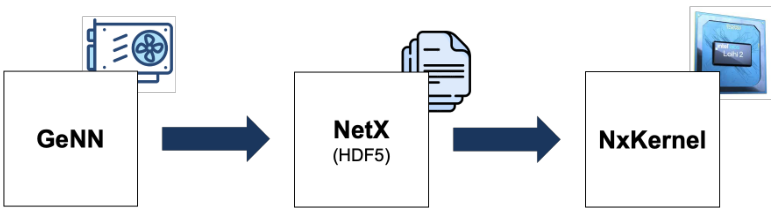
\includegraphics[width=0.62\textwidth]{figs/p1_pipeline.png}
\caption{The deployment pipeline: models are trained with GeNN and exported in the NetX format for inference on Loihi 2 \cite{p1}}
\label{fig:p1_pipeline}
\end{figure}

\begin{algorithm}[htbp]
\caption{Training and deploying delay SNNs on Loihi 2 (summarised from \cite{p1})}\label{alg:p1}
\begin{algorithmic}[1]
\Require spike-encoded dataset (700 input channels); architecture; delay limit $D_{\max}=62$ timesteps
\State Build an LIF network with exponential synapses, weights $w_{ij}$, and delays $d_{ij}$ in mlGeNN
\For{each training epoch}
  \State Simulate the forward pass on the GPU, recording neuron states at spike times
  \State Run the EventProp adjoint backwards in time to obtain exact gradients for $w_{ij}$ and $d_{ij}$
  \State Update weights and delays; regularise hidden firing towards 14 Hz
\EndFor
\State Clamp delays to $d_{ij}<D_{\max}$ and export the network to NetX (HDF5)
\State Quantise weights to 8-bit integers and map the network onto Loihi 2 cores with NxKernel
\State For each input, classify by the output neuron with the largest weighted voltage integral
\end{algorithmic}
\end{algorithm}

\subsection{Network Models and Datasets}

\paragraph{} Two architectures are trained, each with and without delays: a \textbf{single-layer recurrent} network and a \textbf{two-layer feedforward} network of LIF neurons with exponential synapses. Output neurons are non-firing leaky integrators, and the decision is the output with the maximum exponentially weighted voltage integral. Hidden layers have 512 neurons for SHD and 1024 for SSC. Hyperparameter searches covered timesteps of 1--2 ms, delay initialisation ranges, and regularisation strengths, with a target hidden firing rate of 14 Hz; cross-validation on the training set was used for SHD, which has no validation set, and the validation set for SSC \cite{p1}.

\paragraph{} Both datasets come from the Heidelberg spiking data sets of Cramer et al. The \textbf{Spiking Heidelberg Digits} (SHD) contain 10{,}420 spoken digits (0--9) in German and English from 12 speakers. The \textbf{Spiking Speech Commands} (SSC) contain 105{,}829 samples of 35 words from Google Speech Commands, spoken by a larger pool of speakers. In both, audio is converted into spikes on 700 input channels by an artificial cochlea model \cite{p1}.

\subsection{Results and Analysis}

\paragraph{} \textbf{Training efficiency.} Compared with the dilated-convolution method on two-hidden-layer feedforward models, mlGeNN's EventProp delay learning needs only half the memory, even with the 62 delay slots used here, and runs up to 10 times faster \cite{p1}.

\paragraph{} \textbf{Accuracy.} Table~\ref{tab:p1_acc} lists test accuracies with 32-bit floating-point weights in mlGeNN (mean of five seeds) and with 8-bit integer weights on Loihi 2 (one seed). The authors report that delays bring only modest gains for recurrent networks---1.0 percentage points on SHD and 1.6 on SSC---but large gains for feedforward networks, 13.3 points on SHD and 26.9 on SSC, so that the feedforward network with delays achieves the highest SSC accuracy \cite{p1}. Loihi 2 accuracy closely tracks the GPU results, confirming that quantisation to 8-bit costs little; the single-seed Loihi results are even higher in some cases, such as 90.9\% for the recurrent SHD network with delays. Some differences in the GPU columns of the table, such as 72.1\% to 86.9\% for feedforward SHD, are larger than the gains quoted in the text, so the stated percentages should be read as approximate.

{\renewcommand{\arraystretch}{1.15}
\begin{table}[htbp]
\centering
\caption{Test accuracy (\%) of models trained on SHD and SSC \cite{p1}}\label{tab:p1_acc}
\small
\begin{tabular}{|l|l|c|c|c|c|}
\hline
\multirow{2}{*}{\textbf{Dataset}} & \multirow{2}{*}{\textbf{Architecture}} & \multicolumn{2}{c|}{\textbf{mlGeNN (GPU, FP32)}} & \multicolumn{2}{c|}{\textbf{Loihi 2 (INT8)}} \\ \cline{3-6}
 & & No delay & Delay & No delay & Delay \\ \hline
\multirow{2}{*}{SHD} & Feedforward & 72.1 $\pm$ 2.6 & 86.9 $\pm$ 2.3 & 67.9 & 88.0 \\ \cline{2-6}
 & Recurrent & 87.0 $\pm$ 2.1 & 88.8 $\pm$ 2.1 & 89.5 & 90.9 \\ \hline
\multirow{2}{*}{SSC} & Feedforward & 44.5 $\pm$ 1.1 & 71.4 $\pm$ 1.0 & 42.6 & 69.8 \\ \cline{2-6}
 & Recurrent & 63.7 $\pm$ 1.0 & 65.3 $\pm$ 5.7 & 62.5 & 67.8 \\ \hline
\end{tabular}
\end{table}}

\paragraph{} \textbf{Cost of the delay limit.} In the authors' earlier work, models with unconstrained delays outperformed the 62-step models presented here by about 5\% on both datasets. At the 1 ms timestep that gave the best results, 62 steps cover only 62 ms of history, which may be a heavy limitation for keyword recognition \cite{p1}.

\paragraph{} \textbf{Energy and latency.} Table~\ref{tab:p1_energy} compares SHD inference on Loihi 2 with an NVIDIA Jetson Orin Nano. On the Jetson, runtime was measured with CUDA events and power with the \texttt{jtop} tool over the CPU, GPU, CV, and SoC rails, with static power taken from 20 s of idling. At batch size 1 the GPU is under-used and latency is dominated by launching three kernels per timestep, about 10 $\mu$s each, so energy per sample is roughly constant across architectures. Larger batches amortise this overhead and reduce energy per sample by up to 20 times for models without delays, but delayed inputs must be accumulated in global memory and the delay buffers must fit in the 2 MiB L2 cache, so the best batch size for delay models is small and delays cost about 6 times more energy on the Jetson. On Loihi 2, measured on a single-chip Oheo Gulch system in IO-unconstrained mode, delays only marginally increase energy and latency, and the feedforward networks use about 30\% more energy than the recurrent ones because they have twice as many hidden neurons \cite{p1}.

{\renewcommand{\arraystretch}{1.12}
\begin{table}[htbp]
\centering
\caption{SHD inference cost per sample on Loihi 2 and Jetson Orin Nano \cite{p1}}\label{tab:p1_energy}
\small
\setlength{\tabcolsep}{4pt}
\begin{tabular}{|l|c|l|c|c|c|c|}
\hline
\textbf{Arch.} & \textbf{Delay} & \textbf{Hardware} & \textbf{Total (mJ)} & \textbf{Dyn. (mJ)} & \textbf{Lat. (ms)} & \textbf{EDP ($\mu$J$\cdot$s)} \\ \hline
\multirow{6}{*}{FF} & Yes & Jetson, batch 1 & 93.7 & 30.0 & 27.5 & 2581.9 \\
 & No & Jetson, batch 1 & 85.4 & 25.8 & 26.0 & 2219.6 \\
 & Yes & Jetson, batch 4 & 50.6 & 22.6 & 48.5 & 2454.8 \\
 & No & Jetson, batch 128 & 8.3 & 4.9 & 178.8 & 1476.9 \\
 & Yes & Loihi 2 & 0.46 & 0.28 & 1.46 & 0.67 \\
 & No & Loihi 2 & 0.42 & 0.25 & 1.47 & 0.62 \\ \hline
\multirow{6}{*}{Rec} & Yes & Jetson, batch 1 & 93.3 & 29.0 & 27.9 & 2599.0 \\
 & No & Jetson, batch 1 & 85.0 & 25.3 & 26.0 & 2214.8 \\
 & Yes & Jetson, batch 4 & 41.9 & 16.5 & 43.6 & 1827.6 \\
 & No & Jetson, batch 128 & 6.5 & 3.7 & 156.4 & 1018.2 \\
 & Yes & Loihi 2 & 0.36 & 0.21 & 1.54 & 0.56 \\
 & No & Loihi 2 & 0.33 & 0.19 & 1.49 & 0.50 \\ \hline
\end{tabular}
\end{table}}

\paragraph{} At batch size 1, Loihi 2 classifies a sample up to 18 times faster than the Jetson---1.46 ms against 27.5 ms for the feedforward delay network---and uses 200 to 260 times less total energy, the roughly 250-fold reduction quoted by the authors. Even against the Jetson's most efficient batched configurations, which raise latency to as much as 179 ms, Loihi 2 uses 20 to 116 times less energy per sample, and its energy-delay product is more than 2000 times lower \cite{p1}.

\subsection{Discussion}

\paragraph{} The paper's main strength is completeness: it connects a memory-efficient, exact-gradient training method to a real chip and shows that delays, which are expensive on GPUs, are almost free on Loihi 2. It also demonstrates that 8-bit quantisation preserves accuracy. Its limitations are the 62-step delay limit, which costs about 5\% accuracy; the restriction to keyword spotting with fairly large, fully connected layers; Loihi results from a single seed; and an IO-unconstrained measurement mode that excludes the cost of streaming inputs to the chip. The authors propose sparsely connected delay networks, combinations of delays with adaptive or resonate-and-fire neurons, and tasks that need precise timing over long periods as future work \cite{p1}.

% ---------------------------------------------------------------
\section{Accelerating Sensor Fusion in Neuromorphic Computing: A Case Study on Loihi-2}

\paragraph{} Isik, Tiwari, Eryilmaz, and Dikmen \cite{p2}, from Drexel University, IISc Bangalore, Bilkent University, and the Temsa R\&D Center, study whether Loihi-2 can accelerate multimodal sensor fusion for autonomous driving and robotics.

\subsection{Problem Statement and Motivation}

\paragraph{} \textbf{Sensor fusion} integrates data from several sensors---cameras, LIDAR, radar, GPS, inertial measurement units (IMUs), and vehicle buses---to obtain a more accurate and reliable view of the environment than any single sensor provides. Classical approaches include rule-based systems, statistical estimators such as Kalman filters, and neural networks. The task is hard because sensors produce data in different formats and at different rates, calibration discrepancies and noise add uncertainty, data volumes are large, and decisions must be made in real time \cite{p2}. Traditional computing is increasingly strained by these demands, and the authors identify a gap in the literature on applying neuromorphic chips such as Loihi-2 to sensor fusion. Their objectives are to demonstrate Loihi-2's efficacy for sensor fusion and to compare it with conventional CPUs and GPUs.

\subsection{System Architecture}

\paragraph{} Figure~\ref{fig:p2_system} shows the system. A \textbf{host computer} provides visualisation and display control and connects to the chip through a \textbf{communication interface}, such as Ethernet. Loihi-2 sits at the centre, performing sensor fusion and managing input and output, while the sensors act as the system's data sources, sending measurements that are likely encoded as spikes \cite{p2}. Figure~\ref{fig:p2_loop} shows the sensing pipeline for autonomous driving: IMU measurements, angle estimation, CAN-bus data, position estimation, GPS and LIDAR, time synchronisation, and coordinate transformation all feed the fusion stage executed on the neuromorphic unit.

\begin{figure}[htbp]
\centering
\begin{subfigure}[b]{0.52\textwidth}\centering
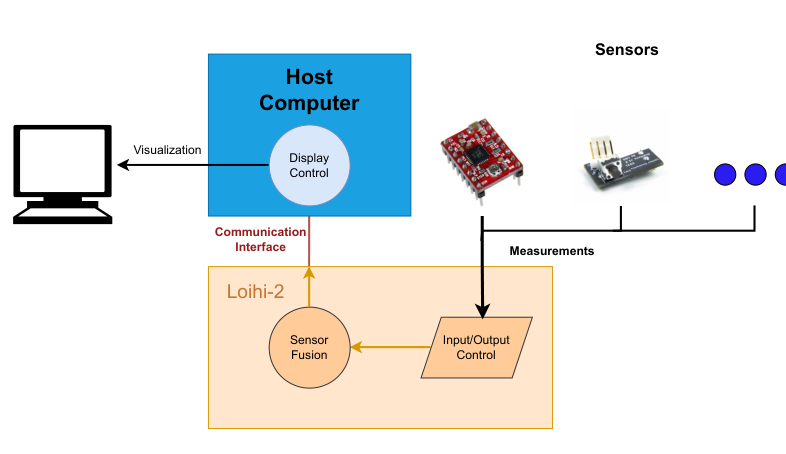
\includegraphics[width=\linewidth]{figs/p2_system.png}
\caption{System architecture}\label{fig:p2_system}
\end{subfigure}\hfill
\begin{subfigure}[b]{0.42\textwidth}\centering
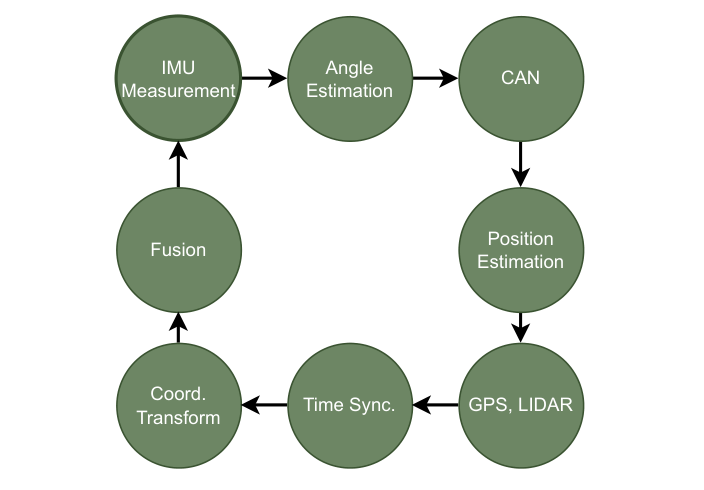
\includegraphics[width=0.85\linewidth]{figs/p2_sensorloop.png}
\caption{Sensing and fusion pipeline}\label{fig:p2_loop}
\end{subfigure}
\caption{System integrating the Loihi-2 chip for sensor fusion, and the processing of camera, LIDAR, radar, GPS, and IMU data for autonomous driving \cite{p2}}
\label{fig:p2_arch}
\end{figure}

\subsection{Datasets}

\paragraph{} Five autonomous-driving datasets, complemented by synthetic data for specific conditions, are used. They differ in sensor modalities and focus, from environmental perception to driver behaviour, which makes them a varied test of multimodal processing \cite{p2}.

\subsection{Implementation Framework}

\paragraph{} Five SNN models, one tailored to each dataset, were first run on conventional CPU and GPU hardware to validate them and then optimised for Loihi-2. Deployment requires generating an \textbf{HDF5} file that captures the trained model's architecture and parameters in a form the Loihi-2 environment accepts, and a script that defines input and output ports and sets up execution on the chip. The authors use \textbf{Lava-DL}, including its SLAYER and Bootstrap libraries, together with \texttt{lava-dl netx}, \texttt{lava.magma.core}, \texttt{lava.process}, and \texttt{lava.util}. A notable practical difficulty was a mismatch between the data loader's output and the input formats expected by Loihi-2, which the authors illustrate with a model trained on CIFAR-10 \cite{p2}.

\paragraph{} The authors place this flow in a broader architecture in which frameworks such as Lava, Neurokernel, PyNN, Brian2, Nengo, and NEURON translate algorithms for neuromorphic execution, communication uses \textbf{NxLink} and \textbf{AER}, and sensors, neuromorphic processing units, and actuators form a closed loop. They also list four practical considerations: exploiting \textbf{sparsity}, \textbf{simplifying neuron models} to fit the chip's dynamics, ensuring \textbf{software--hardware compatibility} with Loihi's software stack, and using Intel's \textbf{neuromorphic debugging tools} \cite{p2}.

\subsection{Results and Analysis}

\paragraph{} \textbf{Hardware comparison.} Table~\ref{tab:p2_hw} compares an Intel i9-12900H CPU, an NVIDIA RTX 3060 GPU, and Loihi 2 running the model for the Oxford Radar RobotCar dataset, with the same 960 million operations per inference on each. Loihi 2 reaches 161.11 GOP/s at only 1.55 W, a power efficiency of \textbf{103.94 GOP/s/W}. The GPU has higher throughput, 304.76 GOP/s, thanks to 3584 cores at 1320 MHz, but draws 80 W, giving 3.80 GOP/s/W, while the CPU achieves 8.67 GOP/s at 28 W, or 0.30 GOP/s/W \cite{p2}. Loihi 2 is therefore about 27 times more power-efficient than the GPU and over 300 times more than the CPU (Figure~\ref{fig:p2_eff}); the authors summarise this as nearly 30 times and over 100 times, respectively.

{\renewcommand{\arraystretch}{1.12}
\begin{table}[htbp]
\centering
\caption{Hardware specifications and results on the Oxford Radar RobotCar model \cite{p2}}\label{tab:p2_hw}
\small
\begin{tabular}{|l|c|c|c|}
\hline
\textbf{Specification} & \textbf{Intel i9-12900H} & \textbf{NVIDIA RTX 3060} & \textbf{Intel Loihi 2} \\ \hline
Technology node & 10 nm & 8 nm & 7 nm (Intel 4) \\ \hline
Core count & 14 & 3584 & 128 \\ \hline
Precision & Float32 & Float32 & Fixed32 \\ \hline
Frequency (MHz) & 3700 & 1320 & 1000 \\ \hline
Memory & DDR5 & GDDR6 & On-chip \\ \hline
MOP per inference & 960 & 960 & 960 \\ \hline
Throughput (GOP/s) & 8.67 & 304.76 & 161.11 \\ \hline
Power (W) & 28 & 80 & 1.55 \\ \hline
Power efficiency (GOP/s/W) & 0.30 & 3.80 & 103.94 \\ \hline
\end{tabular}
\end{table}}

\begin{figure}[htbp]
\centering
\begin{subfigure}[b]{0.48\textwidth}\centering
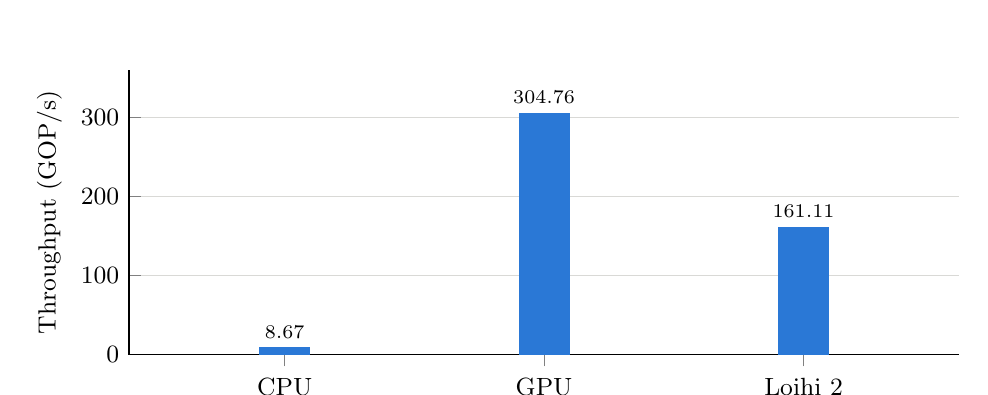
\begin{tikzpicture}
\begin{axis}[ybar, width=\linewidth, height=5.2cm, bar width=18pt, ymin=0, ymax=360,
  symbolic x coords={CPU,GPU,Loihi 2}, xtick=data, enlarge x limits=0.3,
  ylabel={Throughput (GOP/s)}, ymajorgrids, grid style={gridgray}, axis lines*=left,
  nodes near coords, every node near coord/.append style={font=\scriptsize},
  tick label style={font=\small}, label style={font=\small}]
\addplot[fill=seriesA, draw=seriesA] coordinates {(CPU,8.67) (GPU,304.76) (Loihi 2,161.11)};
\end{axis}
\end{tikzpicture}
\caption{Throughput}
\end{subfigure}\hfill
\begin{subfigure}[b]{0.48\textwidth}\centering
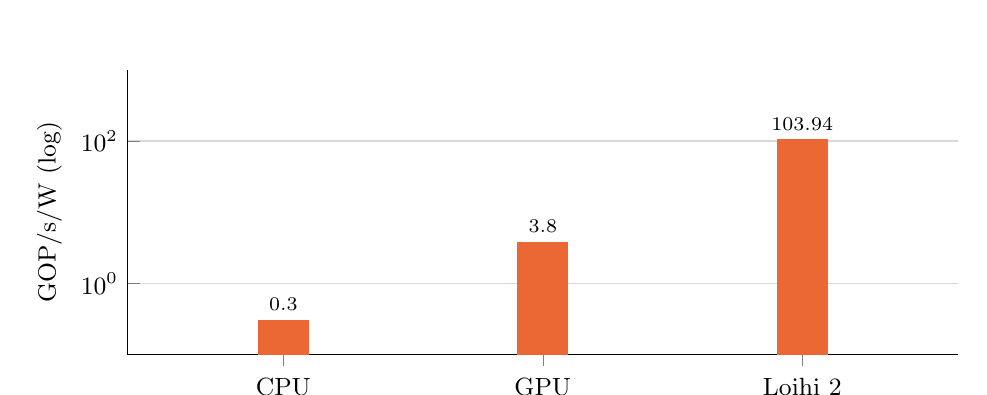
\begin{tikzpicture}
\begin{axis}[ybar, width=\linewidth, height=5.2cm, bar width=18pt, ymode=log, ymin=0.1, ymax=1000, log origin=infty,
  symbolic x coords={CPU,GPU,Loihi 2}, xtick=data, enlarge x limits=0.3,
  ylabel={GOP/s/W (log)}, ymajorgrids, grid style={gridgray}, axis lines*=left,
  nodes near coords, point meta=rawy, every node near coord/.append style={font=\scriptsize},
  tick label style={font=\small}, label style={font=\small}]
\addplot[fill=seriesB, draw=seriesB] coordinates {(CPU,0.30) (GPU,3.80) (Loihi 2,103.94)};
\end{axis}
\end{tikzpicture}
\caption{Power efficiency}
\end{subfigure}
\caption{Throughput and power efficiency of the CPU, GPU, and Loihi 2 on the sensor-fusion model: the GPU is fastest, but Loihi 2 is far more efficient (data from \cite{p2})}
\label{fig:p2_eff}
\end{figure}

\paragraph{} \textbf{Per-dataset performance.} Table~\ref{tab:p2_ds} reports Loihi-2's metrics on all five datasets. The networks use 1100--1200 neurons and 100K--120K synapses, draw 1.5--2.5 W, and complete inference in 0.58--0.80 ms with throughputs of 141--161 GOP/s \cite{p2}. The Oxford Radar RobotCar model is the fastest and most frugal, and the AIODrive model, with the most complex input, is the slowest and most power-hungry. The reported efficiency in pJ per operation does not follow directly from power divided by throughput---for example, 1.50 W at 161 GOP/s gives about 9.3 pJ/op rather than 11.52---so these values are best read as indicative.

{\renewcommand{\arraystretch}{1.12}
\begin{table}[htbp]
\centering
\caption{Performance of Loihi-2 on the five sensor-fusion datasets \cite{p2}}\label{tab:p2_ds}
\small
\setlength{\tabcolsep}{4pt}
\begin{tabular}{|l|c|c|c|c|c|c|}
\hline
\textbf{Dataset} & \textbf{Power (W)} & \textbf{Time (ms)} & \textbf{GOP/s} & \textbf{pJ/OP} & \textbf{Neurons} & \textbf{Synapses} \\ \hline
AIODrive & 2.50 & 0.80 & 141 & 10.12 & 1200 & 120K \\ \hline
Oxford RobotCar & 1.50 & 0.58 & 161 & 11.52 & 1100 & 100K \\ \hline
D-Behavior (D-Set) & 1.78 & 0.61 & 159 & 11.38 & 1100 & 100K \\ \hline
nuScenes & 2.38 & 0.70 & 143 & 10.38 & 1200 & 120K \\ \hline
Comma2k19 & 1.98 & 0.65 & 149 & 11.38 & 1200 & 120K \\ \hline
\end{tabular}
\end{table}}

\paragraph{} \textbf{Comparison with earlier implementations.} The authors compare Loihi-2's inference times with published implementations on FPGAs and GPUs. On nuScenes, earlier systems need 17--700 ms on hardware ranging from an FPGA to RTX 3090 and RTX A6000 GPUs, against 0.70 ms on Loihi-2; on Oxford Radar RobotCar, Burnett et al. need 70 ms on a V100 GPU and Xeon CPU against 0.58 ms; and on D-Set, Liu et al. need 330 ms against 0.61 ms \cite{p2}. On Comma2k19, however, Chen et al. report 0.01 ms on a GTX 1080, faster than Loihi-2's 0.65 ms. The earlier works also solve different, often larger, perception tasks with different models, so these ratios indicate potential rather than like-for-like speed-ups.

\subsection{Discussion}

\paragraph{} The paper is one of the first to apply Loihi-2 to multimodal sensor fusion across several real driving datasets, and it reports sub-millisecond inference at 1.5--2.5 W with power efficiency far above a CPU and GPU. It also shares useful practical lessons on the HDF5/NetX export path and data-format mismatches. Its limitations are significant, however. The SNN architectures, training procedures, and accuracy on each dataset are not reported, so efficiency cannot be weighed against task quality; the experiments use data generated for testing in an ideal environment rather than live sensor streams; several reported figures are internally inconsistent, such as 128 cores and a 7 nm node for an Intel~4 chip that \cite{p1,p4} describe as having 120 cores; and comparisons with earlier implementations mix different tasks. The authors plan real-time sensor fusion experiments and collaboration with industry as future work \cite{p2}.

% ---------------------------------------------------------------
\section{A Spike-Based Long Short-Term Memory on a Neurosynaptic Processor}

\paragraph{} Shrestha, Ahmed, Wang, Widemann, Moody, Van Essen, and Qiu \cite{p3}, from Syracuse University and Lawrence Livermore National Laboratory, present a design flow that maps an LSTM network onto IBM's TrueNorth neurosynaptic processor and evaluate its accuracy, energy, and speed.

\subsection{Problem Statement and Motivation}

\paragraph{} Feedforward networks cannot retain temporal dependencies, and vanilla recurrent networks struggle to learn long dependencies because of vanishing and exploding gradients. The \textbf{LSTM} solves this with gates that control what is forgotten, added to, and output from a cell state, and is a standard model for time-series processing. TrueNorth-compatible learning algorithms had achieved close to state-of-the-art results for feedforward networks such as convolutional networks, but recurrent networks in the spike domain remained at the proof-of-concept level, because of the hardware's limited connectivity and weight precision and the difficulty of capturing recurrent dynamics with asynchronous spiking neurons \cite{p3}. To the authors' knowledge, theirs is the first implementation of an LSTM in the spike domain.

\subsection{LSTM and the TrueNorth Architecture}

\paragraph{} A standard LSTM computes, at each step $t$,
\begin{equation}
\begin{aligned}
f_t&=\sigma\big(W_f[h_{t-1},x_t]+b_f\big), & i_t&=\sigma\big(W_i[h_{t-1},x_t]+b_i\big),\\
C'_t&=\tanh\big(W_C[h_{t-1},x_t]+b_C\big), & C_t&=f_t\ast C_{t-1}+i_t\ast C'_t,\\
o_t&=\sigma\big(W_o[h_{t-1},x_t]+b_o\big), & h_t&=o_t\ast\tanh(C_t),
\end{aligned}
\end{equation}
where $f_t$, $i_t$, and $o_t$ are the forget, input, and output gates, $C_t$ is the cell state, and $h_t$ is the output \cite{p3}. Implementing these equations requires matrix--vector products, two non-linearities, element-wise products, and a sum, all synchronised so that $h_{t-1}$ meets $x_t$ at the right moment. On TrueNorth (Figure~\ref{fig:p3_core}), each core is a crossbar of 256 axons and 256 neurons; a group of cores with defined inputs and outputs forms a \textbf{corelet}, and corelets are composed into larger networks.

\begin{figure}[htbp]
\centering
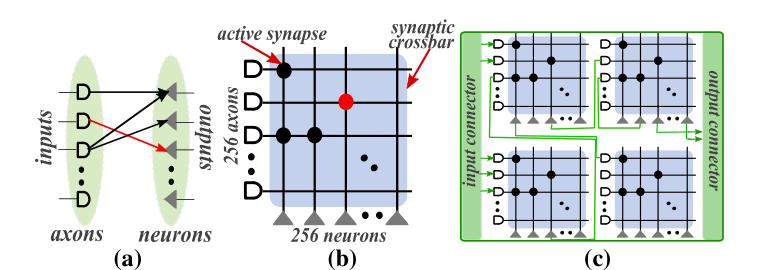
\includegraphics[width=0.62\textwidth]{figs/p3_core.png}
\caption{(a) Structural view, (b) crossbar view, and (c) corelet abstraction of a TrueNorth core \cite{p3}}
\label{fig:p3_core}
\end{figure}

\subsection{Constrain-Then-Train-Then-Approximate}

\paragraph{} TrueNorth weights are low-precision integers with at most four values per neuron, and the authors found that LSTMs are hard to train with binary or ternary weights. They therefore train a regular LSTM under constraints that anticipate the hardware and then approximate it, a process they call \textbf{constrain-then-train-then-approximate}. Weights are constrained to $[-1,1]$ or $[-2,2]$ during training so that they can later be scaled into the hardware range, and the gates are replaced by piecewise-linear versions with steep slopes,
\begin{equation}
\sigma(x)=\max\big(0,\min(1,\,x+0.5)\big),\qquad \tanh(x)=\max\big(-1,\min(1,\,2x)\big),
\end{equation}
which are used during both training and recall. After training, the floating-point weights are scaled and rounded to the hardware precision \cite{p3}. The steep slopes shrink the linear range of the gates and limit the propagation of rounding errors.

\subsection{Spike Encoding}

\paragraph{} LSTM values can be negative, but spikes are binary. Replacing $\tanh$ with ReLU would make all values positive, but unbounded activations can make an LSTM diverge, so the authors instead use separate \textbf{positive and negative spike channels}. Inputs and outputs are \textbf{rate-coded} over a window called the \textbf{phase length} (PL). If $mx$ is the maximum value to represent and the weights are scaled up by a factor $sf$, the number of spikes that represents the value 1 is
\begin{equation}
nS=\frac{PL}{mx\cdot sf},
\end{equation}
a value $I_v$ is sent at a firing rate of $I_v\cdot nS/PL$, and $n$ spikes received in a phase represent $\mathit{RPValue}=n/nS$. Each spike is therefore worth $1/nS$, so precision improves with the phase length. All internal variables are rate-coded except the cell state $C_t$: because errors in $C_t$ accumulate through its feedback loop, it is represented with a \textbf{burst code}, whose spike count correlates much more closely with the value than a stochastic rate code \cite{p3}.

\subsection{Store-and-Release Synchronisation}

\paragraph{} Asynchronous neurons fire as soon as they can, but an LSTM needs its gates to operate on synchronised inputs. The authors solve this with a \textbf{store-and-release} mechanism. A store-and-release neuron has a large negative, saturating threshold and two clock inputs. A spike on the \emph{store} clock, with a large negative weight, pushes the membrane potential to the negative threshold; the neuron then accumulates input spikes without firing. A spike on the \emph{release} clock, with a large positive weight, raises the potential to zero or above, and the neuron emits spikes in proportion to what it stored. Because a saturated neuron cannot count negative inputs, a \emph{pre-charge} spike on the release line first lifts the potential to an intermediate level; Figure~\ref{fig:p3_sr} shows a neuron entering store mode through $-250$ and release through two pulses of $+100$ \cite{p3}. During release, the accumulated membrane potential (AMP) equals the net number of stored input spikes; at each tick a random number in $[0,R_{ThR}]$ is drawn and a spike is emitted if it is below the AMP, so about $PL\cdot\mathit{AMP}/R_{ThR}$ spikes are produced, and with $R_{ThR}=PL$ the neuron simply relays its input.

\begin{figure}[htbp]
\centering
\begin{subfigure}[b]{0.50\textwidth}\centering
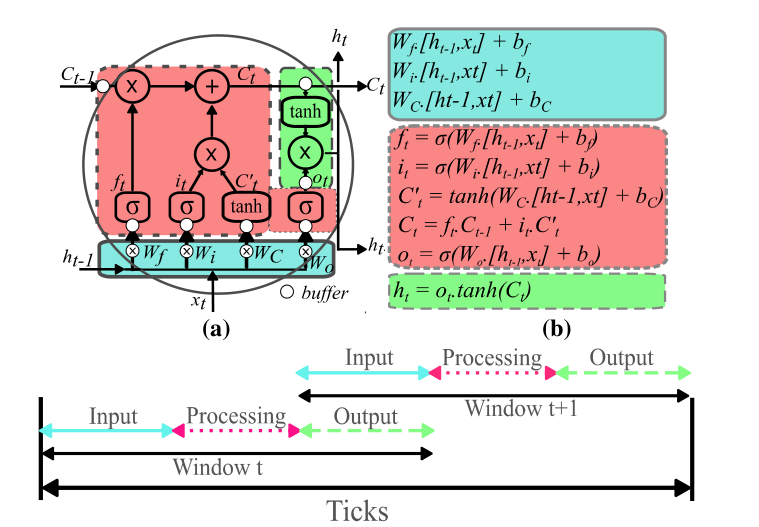
\includegraphics[width=\linewidth]{figs/p3_phases.png}
\caption{Partitions, phases, and partial pipelining}\label{fig:p3_phases}
\end{subfigure}\hfill
\begin{subfigure}[b]{0.46\textwidth}\centering
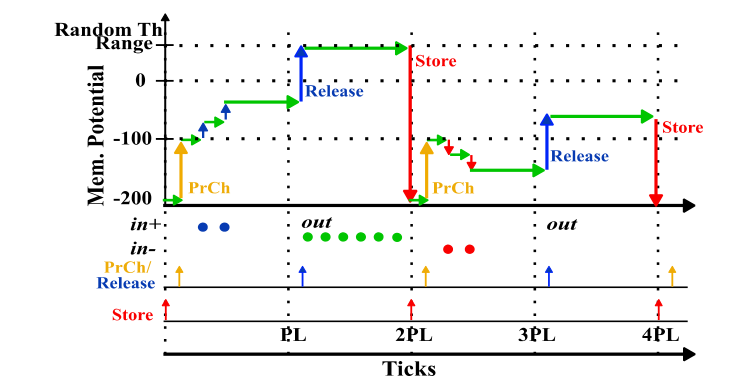
\includegraphics[width=\linewidth]{figs/p3_storerelease.png}
\caption{Store-and-release neuron}\label{fig:p3_sr}
\end{subfigure}
\caption{Operation of the spike-based LSTM: input (blue), processing (red), and output (green) partitions alternate between phases, synchronised by store-and-release neurons driven by store, pre-charge, and release clocks \cite{p3}}
\label{fig:p3_sync}
\end{figure}

\paragraph{} With this mechanism the S-LSTM works in two alternating phases (Figure~\ref{fig:p3_phases}). In the \textbf{I/O phase}, the input partition computes the matrix--vector products for the three gates and the candidate state, and the results are buffered by store-and-release neurons. In the \textbf{processing phase}, these neurons release their contents and the processing partition computes the new cell state $C_t$ and the partial output, which are buffered in turn. In the next I/O phase they are released to compute $h_t$, which is fed back to the input partition together with the next input $x_{t+1}$. The phases are driven by locally generated but globally consistent clock spikes, and the partitions are partially pipelined \cite{p3}.

\subsection{Constituent Modules and Mapping}

\paragraph{} Each part of the LSTM becomes a parameterised corelet. The \textbf{Input Collection (IC) module} performs the matrix--vector products: every input uses two channels, and each weight is formed by four axons with weights 1, 2, 4, and 8, approximating values from $-15$ to $+15$---5-bit rather than 4-bit precision thanks to the two channels---with the product routed to the positive or negative output according to its sign. The \textbf{sigmoid} and \textbf{tanh modules} are store-and-release neurons whose release rates implement the hard functions above: the sigmoid adds an offset of $nS/2$ to the accumulated potential and uses $R_{ThR}=nS$, and the tanh uses two output channels with $R_{ThR}=nS/2$. The \textbf{dot-product module} multiplies the burst-coded cell state by a stochastically rate-coded sigmoid output through a logical AND of the two spike trains, realised by an integrate-and-fire neuron with threshold 2: in a 10-tick window, 5 sigmoid spikes (0.5) and 4 input spikes (0.4) yield 2 output spikes (0.2) \cite{p3}.

\paragraph{} Because a core has only 256 axons and 256 neurons, the modules are placed by an \textbf{incremental mapping algorithm} that adds a new core only when the current one is full. IC modules grow along both axons and neurons, since their size depends on the numbers of inputs and hidden units, whereas the other modules grow only along axons. Cores are therefore added in steps, and the average number of neurons used per core rises with network size \cite{p3}.

\subsection{Experiments and Results}

\paragraph{} All networks have one hidden LSTM layer, are trained with weights constrained to $[-2,2]$, and use $mx=5$; the Keras/TensorFlow counterparts reach 100\% accuracy in every case \cite{p3}. Two benchmarks are used. In the \textbf{parity check} problem, the network reads a binary sequence and reports after each bit whether the number of ones so far is even or odd; LSTMs with 2, 4, and 10 units are trained on 9000 sequences of up to 20 bits and tested on 1000 sequences on TrueNorth. In the \textbf{Embedded Reber Grammar} (ERG) task, the network reads symbols generated by walking a grammar graph and predicts the possible next symbols, coded as 7-dimensional binary vectors; LSTMs with 10, 30, and 50 units are trained on 5000 sequences of up to 36 symbols and tested on 500.

\begin{figure}[htbp]
\centering
\begin{subfigure}[b]{0.48\textwidth}\centering
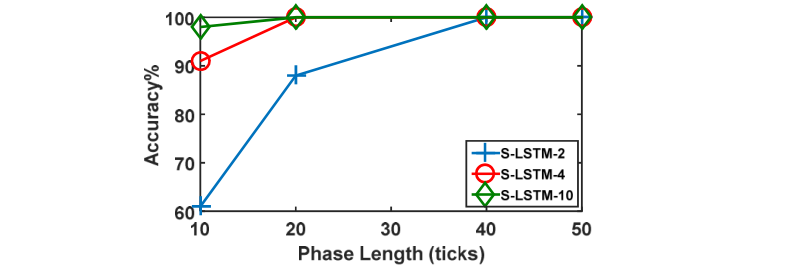
\includegraphics[width=\linewidth]{figs/p3_parity.png}
\caption{Parity check (2, 4, and 10 units)}\label{fig:p3_parity}
\end{subfigure}\hfill
\begin{subfigure}[b]{0.48\textwidth}\centering
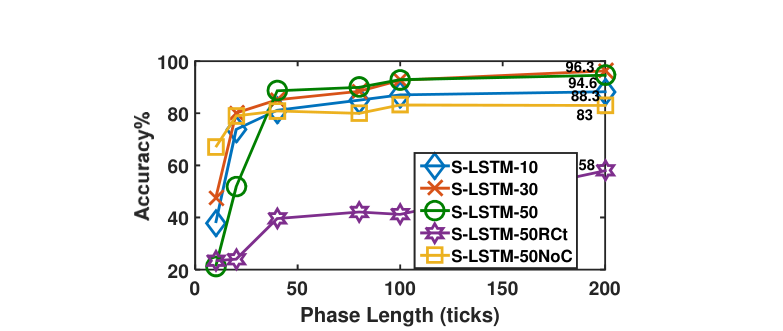
\includegraphics[width=\linewidth]{figs/p3_erg.png}
\caption{Embedded Reber grammar}\label{fig:p3_erg}
\end{subfigure}
\caption{Accuracy of the spike-based LSTM on TrueNorth versus phase length; RCt denotes a rate-coded cell state and NoC a network trained without weight constraints \cite{p3}}
\label{fig:p3_acc}
\end{figure}

\paragraph{} \textbf{Accuracy.} Figure~\ref{fig:p3_acc} shows that accuracy rises with phase length, which increases the precision of activations, and with the number of LSTM units. On parity, the 10-unit network is nearly perfect from a phase length of 10 ticks and reaches 100\% at 20, whereas the 2-unit network needs 40 ticks. On ERG, accuracy improves sharply once precision exceeds $1/10$, and at a phase length of 200 ticks the 50-unit network reaches 96.3\%. Two ablations explain the design choices. A rate-coded cell state (S-LSTM-50RCt) reaches only 58\%, because rounding and sampling errors accumulate around the feedback loop. A network trained without constraints (S-LSTM-50NoC) is more accurate at short phase lengths, since its scaling factor $sf=1$ gives a higher $nS$, but it plateaus at 83\%, below the constrained network, once long windows provide enough precision \cite{p3}.

\paragraph{} \textbf{Energy.} Active power on TrueNorth is the measured total minus the leakage power, and leakage is scaled by the fraction of the chip's 4096 cores that the network uses, so packing neurons densely onto few cores matters. The 10-, 30-, and 50-unit networks use 17, 18, and 28 cores, with neuron density per core increasing with size. Table~\ref{tab:p3_power} compares the 50-unit network with GPU implementations. At its normal 1 kHz tick and 0.8 V, TrueNorth needs only \textbf{56 $\mu$J} per sample at a phase length of 200, which is 84 times more energy-efficient than an NVIDIA Tegra X1 and 416 times more than a Titan X. Running 3.5 times faster than real time at the same voltage improves this to 165 and 817 times \cite{p3}.

{\renewcommand{\arraystretch}{1.12}
\begin{table}[htbp]
\centering
\caption{Power and performance of a 50-unit LSTM on different platforms \cite{p3}}\label{tab:p3_power}
\small
\begin{tabular}{|l|c|c|c|}
\hline
\textbf{Device} & \textbf{Time/sample (ms)} & \textbf{Power (W)} & \textbf{Energy (mJ)} \\ \hline
NVIDIA Tegra X1 & 1.928 & 2.45 & 4.72 \\ \hline
NVIDIA Titan X & 0.5 & 46.5 & 23.3 \\ \hline
TrueNorth (PL = 200) & 400 & 0.00014 & 0.056 \\ \hline
TrueNorth, 3.5$\times$ real time & 114 & 0.00025 & 0.0285 \\ \hline
\end{tabular}
\end{table}}

\paragraph{} \textbf{Latency trade-off.} TrueNorth is, however, much slower: 400 ms per sample against 1.9 ms on the Tegra X1 and 0.5 ms on the Titan X. The authors attribute this mainly to the inability to train LSTMs reliably with very low precision, which forces a long phase length to reach good accuracy; a network trained for very limited precision could use $sf=1$ and much shorter phases, bringing latency close to that of GPUs at the same or lower energy \cite{p3}.

\subsection{Discussion}

\paragraph{} The paper's strengths are its modular, reusable design---corelets for each LSTM component that can be applied to other spiking platforms---and its careful handling of synchronisation, signed values, and precision under severe hardware constraints, yielding energy two to three orders of magnitude below GPUs. Its limitations are the small benchmarks, latency hundreds of times longer than GPUs, accuracy below the floating-point model at practical phase lengths, and a single hidden layer. It nevertheless anticipates two ideas found in later work: exploiting temporal precision through spike timing \cite{p1} and carrying exact values in spikes rather than rates \cite{p4}.

% ---------------------------------------------------------------
\section{Sigma-Delta Neural Network Conversion on Loihi 2}

\paragraph{} Brehove, Tumpa, Kyubwa, Menon, and Narayanan \cite{p4}, from ChromoLogic LLC and Pennsylvania State University, convert conventionally trained and quantised neural networks into sigma-delta neural networks that run on Loihi 2, benchmark them against NVIDIA Jetson boards, and deploy one in a field exercise.

\subsection{Problem Statement and Motivation}

\paragraph{} Training SNNs directly to accuracies comparable to deep ANNs is difficult because the loss must be backpropagated through time; in the authors' experiments, training a spiking network took about 10 times as long as training an ANN of the same architecture. Classic ANN-to-SNN conversion uses spike rates to represent activations and therefore needs many timesteps per input, which erodes efficiency \cite{p4}. Intel's earlier sigma-delta networks on Loihi 2 relied on SLAYER, which stores the whole time series during training and is slower than conventional training, and an earlier conversion method by Yousefzadeh et al. used binary spikes and was incompatible with modern quantisation. The goal is therefore a conversion path that starts from standard PyTorch training and quantisation and produces sparse networks that exploit Loihi 2's graded spikes.

\subsection{Sigma-Delta Neurons and the Conversion Method}

\paragraph{} A \textbf{sigma-delta neuron} \cite{oconnor2016} receives spikes that represent \emph{changes} in the previous layer's activations, multiplies them by its weights, adds them to a running sum, and sends the change in its own activation to the next layer only if that change exceeds a threshold (Figure~\ref{fig:p4_neuron}). Apart from this, it behaves exactly like a conventional ANN neuron, but because it computes only when inputs change, it naturally exhibits temporal sparsity, and because only some neurons change at a time it also exhibits spatial sparsity \cite{p4}.

\begin{figure}[htbp]
\centering
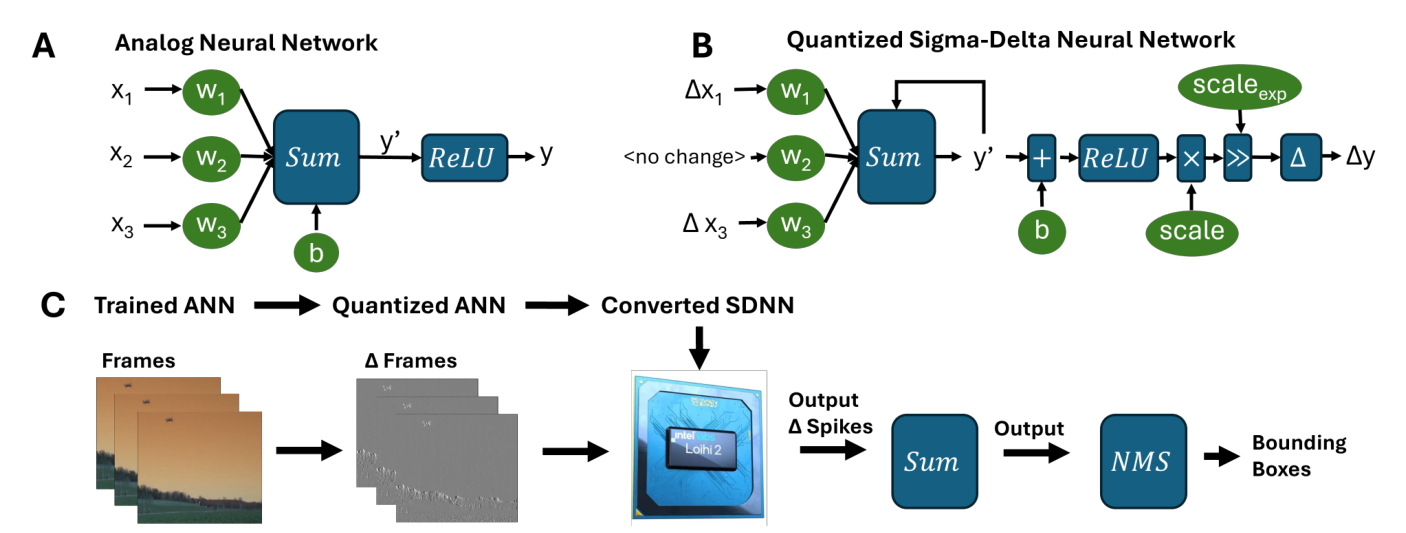
\includegraphics[width=0.95\textwidth]{figs/p4_neuron.png}
\caption{(A) A conventional ANN neuron; (B) a quantised sigma-delta neuron on Loihi 2, which accumulates weighted input changes, applies ReLU and integer rescaling, and emits a graded spike $\Delta y$ when its output has changed by more than a threshold; (C) the workflow from trained ANN to quantised ANN to converted SDNN, with frames turned into delta spikes and output spikes summed into bounding boxes \cite{p4}}
\label{fig:p4_neuron}
\end{figure}

\paragraph{} Loihi 2's neurocores compute only with integers, so the network must be quantised. The authors use PyTorch's \textbf{post-training static quantisation}, which converts weights and activations from FP32 to 8-bit integers with an affine mapping $x_{\mathrm{float}}=s\,(x_q-z)$ defined by a floating-point scale $s$ and an integer zero point $z$, while biases stay in FP32. A layer's floating-point output is then
\begin{equation}
y_{\mathrm{float},j}=\sum_{k}\big(x_{q,k}-z_x\big)\big(w_{q,jk}-z_w\big)\,s_x\,s_w+b_{\mathrm{float},j},
\end{equation}
and must be re-quantised with the output scale $s_y$ for the next layer. Intel's original sigma-delta microcode could rescale only by powers of two, so the authors \textbf{redesigned the neuron microcode}: the 24-bit accumulated pre-activation is multiplied by a pre-computed 24-bit integer \emph{scale} derived from $s_x s_w/s_y$ and right-shifted by a pre-computed exponent, $y=(\mathit{acc}\times\mathit{scale})\gg\mathit{scale}_{\exp}$, which keeps the result within 8 bits and prevents overflow in the next layer's 24-bit accumulator, following the integer-only inference approach of Jacob et al. \cite{p4}. Algorithm~\ref{alg:p4} gives the new neuron logic.

\begin{algorithm}[htbp]
\caption{Redesigned sigma-delta neuron microcode on Loihi 2 \cite{p4}}\label{alg:p4}
\begin{algorithmic}[1]
\Require quantised weights $w_q$; rescaled bias; integer \emph{scale} and \emph{scale}$_{\exp}$; threshold $v_{th}$
\State $y'\gets y'+\Delta x\cdot w_q$ \Comment{accumulate weighted input delta}
\State $y\gets\mathrm{ReLU}(y'+\mathit{bias})$
\State $y\gets(y\times\mathit{scale})\gg\mathit{scale}_{\exp}$ \Comment{fixed-point rescaling}
\State $\Delta y\gets y-y_{\mathrm{ref}}$
\If{$|\Delta y|>v_{th}$}
  \State emit graded spike carrying $\Delta y$; $y_{\mathrm{ref}}\gets y$
\EndIf
\end{algorithmic}
\end{algorithm}

\paragraph{} At run time, an initial \textbf{delta layer} on the host CPU turns a sequence of RGB frames into graded spikes, $\mathit{spike}_i=\mathit{frame}_i-\mathit{frame}_{i-1}$. Loihi 2 performs the convolutions and sigma-delta neurons, and its output spikes are added to a running sum on the host, dequantised with the final layer's scale, and interpreted as a YOLOv3-style grid of $14\times14$ cells, each with locations and scores for three bounding boxes. Deployment uses \texttt{nxkernel} v0.3.0 in \textbf{fall-through mode}, which runs 16 SNN timesteps per input so that each frame propagates through the whole network, trading a little throughput for much lower latency than the pipelined mode \cite{p4}.

\subsection{Datasets, Models, and Training}

\paragraph{} Two applications are used. \textbf{Drone detection} uses the Multi-Sensor Drone Detection (MSDD) dataset: 285 RGB videos at $640\times512$, resized to $448\times448$, with four labelled classes---drones, airplanes, helicopters, and birds---at 20--200 m in daylight, with 20\% held out for testing. Ground-based sky videos have few moving objects, so they are highly temporally sparse. \textbf{Steering-angle prediction} uses the Driving dataset, on which Intel demonstrated SLAYER-trained SDNNs; dashboard frames are resized to $66\times200\times3$ for PilotNet \cite{p4}. Table~\ref{tab:p4_models} summarises the models. YOLO-KP, developed by Intel from YOLOv3-Tiny, was adapted to Loihi 2's memory limits by replacing max-pooling with strided convolutions and removing residual layers, which also avoids synchronising spikes from different layers; PilotNet is identical to Intel's SLAYER-trained model.

{\renewcommand{\arraystretch}{1.12}
\begin{table}[htbp]
\centering
\caption{Models converted and deployed on Loihi 2 \cite{p4}}\label{tab:p4_models}
\small
\begin{tabular}{|l|c|c|}
\hline
 & \textbf{PilotNet} & \textbf{YOLO-KP} \\ \hline
Type & Conv/FC & Conv \\ \hline
Application & Steering-angle prediction & Object detection \\ \hline
Parameters & 0.35M & 3.4M \\ \hline
Neurons & 12K & 2M \\ \hline
Loihi 2 chips & 1 & 5 \\ \hline
\end{tabular}
\end{table}}

\paragraph{} To show that conversion works with any standard training recipe, YOLO-KP is trained by \textbf{knowledge distillation} from a MobileNetV2 teacher, combining the detection loss with a masked L2 feature-matching loss on the penultimate layer weighted by $\alpha=0.069$, with Optuna hyperparameter tuning, albumentations augmentation, the Adam optimiser, and 30 epochs. The model is then quantised to 8-bit per tensor. Sparsity is controlled by the sigma-delta \textbf{threshold}: with a threshold of zero, the cumulative output exactly matches the quantised network, and raising it from 0 to 4 passes only larger changes, reducing spikes and synaptic operations at some cost in accuracy \cite{p4}.

\paragraph{} Loihi 2 is benchmarked on an in-house VPX board with 16 chips, using NxKernel's probes for power, timing, and core activity; static power is counted only for the chips the network uses, and the EDP combines energy and latency. To separate computation from input/output (IO), 100 frames are also loaded into on-chip memory and replayed 10{,}000 times. The baseline runs the same network as a 16-bit floating-point ANN with TensorRT on a Jetson Xavier at batch size 1, measuring whole-SoC power with \texttt{tegrastats}; the authors note that this is not an identical comparison, since only the Loihi 2 chips' power is counted \cite{p4}.

\subsection{Results and Analysis}

\paragraph{} \textbf{Accuracy and training.} The MobileNetV2 teacher reaches 0.72 mAP and the distilled YOLO-KP student 0.74, whereas YOLO-KP without distillation never exceeded 0.6; after 8-bit quantisation the student scores 0.62 mAP over 58 test videos with 18{,}214 frames. PilotNet reaches its lowest MSE, 0.0278, at threshold 0 \cite{p4}. Against SLAYER training of the same YOLO-KP SDNN, the conversion approach is both more accurate and far faster to train: 5 minutes per epoch and 3.4 hours in total against 55 minutes and 45.8 hours, with 8.6 GB instead of 9.4 GB of memory and 0.62 instead of 0.37 mAP; conversion itself adds only 30 seconds of post-training quantisation.

\paragraph{} \textbf{YOLO-KP efficiency.} Sweeping the threshold shows the sparsity trade-off. At threshold 0 the SDNN performs only 0.056 of the ANN's operations, an 18-fold sparsity gain; raising the threshold to 4 increases this to 250-fold and throughput from 176 to 362 FPS, while mAP falls. Loihi 2's power stays roughly constant because it is dominated by static draw. At threshold 0 (Table~\ref{tab:p4_perf}), Loihi 2 uses 11.73 mJ per frame with 3.20 ms latency, against 14.10 mJ and 3.11 ms on the Jetson Xavier, giving a modestly lower EDP but lower throughput \cite{p4}.

{\renewcommand{\arraystretch}{1.12}
\begin{table}[htbp]
\centering
\caption{Loihi 2 compared with Jetson boards at zero threshold \cite{p4}}\label{tab:p4_perf}
\small
\setlength{\tabcolsep}{4pt}
\begin{tabular}{|l|l|c|c|c|c|}
\hline
\textbf{Model} & \textbf{Platform} & \textbf{mJ/frame} & \textbf{Latency (ms)} & \textbf{FPS} & \textbf{EDP ($\mu$J$\cdot$s)} \\ \hline
YOLO-KP SDNN & Loihi 2 & 11.73 & 3.20 & 175.6 & 37.59 \\ \hline
YOLO-KP SDNN & Loihi 2, no IO & 19.89 & 2.86 & 196.5 & 56.93 \\ \hline
YOLO-KP ANN & Jetson Xavier & 14.10 & 3.11 & 321.9 & 43.80 \\ \hline
PilotNet SDNN & Loihi 2 & 1.31 & 2.50 & 200.2 & 3.26 \\ \hline
PilotNet SDNN & Loihi 2, no IO & 1.06 & 1.13 & 442.9 & 1.20 \\ \hline
PilotNet ANN & Jetson Nano & 21.94 & 5.77 & 173.2 & 126.20 \\ \hline
\end{tabular}
\end{table}}

\paragraph{} \textbf{PilotNet efficiency.} For PilotNet, the SDNN on Loihi 2 needs 1.31 mJ per frame and 2.50 ms, against 21.94 mJ and 5.77 ms for the ANN on a Jetson Nano, so energy is about \textbf{16 times} lower and EDP about \textbf{40 times} lower (3.26 against 126.20 $\mu$J$\cdot$s). Without IO, energy falls to 1.06 mJ, latency to 1.13 ms, and throughput rises to 442.9 FPS, giving an EDP of 1.20 $\mu$J$\cdot$s, about 105 times below the Jetson. Re-running Intel's own PilotNet SDNN with the newer NxKernel API showed similar energy to Intel's published 1.26 mJ but far lower latency than its 65.4 ms, indicating that IO and system overheads dominated the earlier pipeline. The converted PilotNet also achieves a lower MSE than the SLAYER-trained equivalent, although with somewhat less sparsity, since conversion does not explicitly encourage sparsity during training \cite{p4}.

\paragraph{} \textbf{Field deployment.} To test operational feasibility, YOLO-KP was trained as an ANN on the infrared subset of MSDD, converted, and deployed on the Loihi 2 VPX board at the US Navy's \textbf{Silent Swarm 2025} exercise (Figure~\ref{fig:p4_field}). The host quantised and delta-encoded frames, sent spikes to Loihi 2 over Ethernet, and summed the output spikes for non-maximum suppression and display. The system ran in real time at \textbf{112 FPS} with \textbf{5.0 ms} latency and \textbf{20 mJ} per frame. Detection reflected a large domain gap: the MSDD model scored 0.03 mAP on the exercise data, rising tenfold to 0.30 mAP after minimal fine-tuning on a small subset. Novel drone types, more complex backgrounds, and camera motion reduced temporal sparsity, with 13\% of inputs non-zero after delta encoding against 2\% for MSDD \cite{p4}.

\begin{figure}[htbp]
\centering
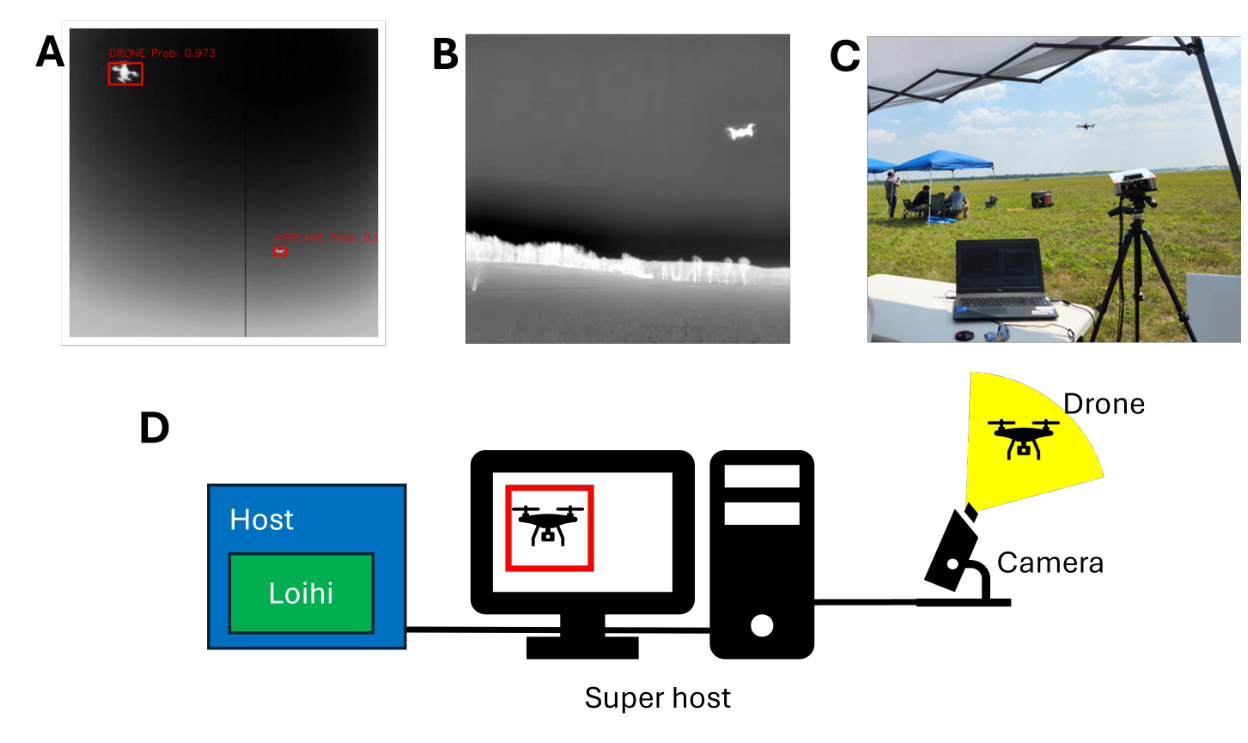
\includegraphics[width=0.72\textwidth]{figs/p4_field.png}
\caption{Field deployment at Silent Swarm 2025: (A) infrared frame with a drone and an airplane, (B) a training frame from MSDD, (C) the field setup with an IR camera and the Loihi 2 VPX board, and (D) the system diagram \cite{p4}}
\label{fig:p4_field}
\end{figure}

\subsection{Discussion}

\paragraph{} The work's main strength is practicality: it lets developers use the ordinary PyTorch toolchain---optimisers, augmentation, distillation, and quantisation---and still obtain sparse networks that run on Loihi 2, with better accuracy and an order of magnitude faster training than SLAYER, and it validates the result in a live field deployment. Its limitations are that gains depend strongly on temporal sparsity, being large for PilotNet but modest for YOLO-KP, whose throughput is lower than the Jetson's; that Loihi 2's on-chip SRAM raises static power, which grows with the number of chips needed for high-resolution inputs; and that the Jetson comparisons use whole-SoC power and, for PilotNet, Intel's earlier measurements. The authors suggest pairing SDNNs with event-based cameras and using larger single chips to reduce costly inter-chip communication \cite{p4}.

% ---------------------------------------------------------------
\section{Summary of the Reviewed Papers}

\paragraph{} Table~\ref{tab:summary} summarises the four works; the next chapter compares them in detail.

{\renewcommand{\arraystretch}{1.15}
\begin{table}[htbp]
\centering
\caption{Summary of the reviewed works}\label{tab:summary}
\small
\begin{tabularx}{\textwidth}{|p{2.2cm}|p{2.5cm}|X|X|}
\hline
\textbf{Work} & \textbf{Problem} & \textbf{Technique} & \textbf{Headline result} \\ \hline
Meszaros et al. \cite{p1} & Keyword spotting on Loihi 2 & EventProp delay learning in mlGeNN, NetX export, NxKernel deployment & Up to 26.9-point accuracy gain from delays; up to 18$\times$ faster and $\sim$250$\times$ less energy than Jetson Orin Nano \\ \hline
Isik et al. \cite{p2} & Multimodal sensor fusion for driving & Five dataset-specific SNNs with Lava-DL on Loihi-2 & 103.94 GOP/s/W; 0.58--0.80 ms inference at 1.5--2.5 W \\ \hline
Shrestha et al. \cite{p3} & Recurrent networks on TrueNorth & Constrain-train-approximate LSTM; burst-coded cell state; store-and-release & 56 $\mu$J/sample; 84--817$\times$ more efficient than GPUs \\ \hline
Brehove et al. \cite{p4} & Efficient ANN-to-SNN deployment & Quantised ANN to sigma-delta SNN with redesigned microcode & PilotNet 16$\times$ lower energy, $\sim$40$\times$ lower EDP; field deployment at 112 FPS \\ \hline
\end{tabularx}
\end{table}}

% ================= CHAPTER 4: DISCUSSION & COMPARISON =================
\chapter{Discussion \& Comparison}

\paragraph{} This chapter compares the four reviewed works. All deploy spiking networks on neuromorphic processors and compare them with conventional hardware, but they differ in how they obtain the network, how they encode information, which chip they target, and how they measure efficiency. The comparison highlights their complementary strengths and the trade-offs among accuracy, energy, latency, and ease of use.

\section{Analytical Focus and Methodology}

\paragraph{} The works examine neuromorphic deployment from four angles: \textbf{learning temporal structure} through trainable delays and bringing it to the chip \cite{p1}; the \textbf{system-level benefit} of neuromorphic hardware for a demanding multimodal application \cite{p2}; \textbf{building a complex recurrent architecture} from spiking circuits under severe hardware constraints \cite{p3}; and \textbf{reusing the conventional deep-learning toolchain} through conversion \cite{p4}. Together they cover the path from training algorithm to field deployment. Table~\ref{tab:cmp_method} compares their methodologies.

{\renewcommand{\arraystretch}{1.15}
\begin{table}[htbp]
\centering
\caption{Methodological comparison of the reviewed works}\label{tab:cmp_method}
\small
\begin{tabularx}{\textwidth}{|p{2.2cm}|X|X|X|X|}
\hline
\textbf{Aspect} & \textbf{Meszaros et al. \cite{p1}} & \textbf{Isik et al. \cite{p2}} & \textbf{Shrestha et al. \cite{p3}} & \textbf{Brehove et al. \cite{p4}} \\ \hline
Hardware & Loihi 2 (1 chip) & Loihi-2 & TrueNorth & Loihi 2 (1--5 chips) \\ \hline
Network & FF and recurrent LIF SNN & Five dataset-specific SNNs & One-layer LSTM & YOLO-KP, PilotNet \\ \hline
How obtained & Direct EventProp training & Lava-DL training, NetX export & Constrain, train, approximate & Quantised ANN conversion \\ \hline
Coding & Binary spikes, delays & Binary spikes & Rate and burst codes & Graded sigma-delta spikes \\ \hline
Task & Keyword spotting & Sensor fusion & Parity, Reber grammar & Detection, steering \\ \hline
Baseline & Jetson Orin Nano & i9 CPU, RTX 3060 GPU & Tegra X1, Titan X & Jetson Xavier, Nano \\ \hline
Accuracy reported & Yes & No & Yes & Yes \\ \hline
\end{tabularx}
\end{table}}

\section{Training and Conversion Strategies}

\paragraph{} The works illustrate the main routes to a deployable SNN. \textbf{Direct training} \cite{p1} gives the most freedom: EventProp learns weights and delays jointly with exact gradients and produces networks that genuinely compute in time, but it needs a specialised toolchain---mlGeNN, NetX, and NxKernel. \textbf{Constrain-then-train-then-approximate} \cite{p3} uses conventional training but needs hand-designed circuits, and residual approximation errors must be paid for with long phase lengths. \textbf{Conversion} \cite{p4} is the most accessible: any PyTorch model that can be quantised can, in principle, run on Loihi 2, and it trained 11 times faster per epoch than SLAYER with higher mAP. Paper \cite{p2} uses the Lava-DL route and documents its practical friction. The more a method reuses standard tools, the easier it is to adopt, but the less it exploits uniquely spiking features such as delays.

\section{Neural Coding and Sparsity}

\paragraph{} Coding determines how many spikes---and therefore how much energy---a computation needs. Rate coding \cite{p3} needs many spikes per value, which is why the S-LSTM needs 200-tick phases and 400 ms per sample, although burst coding improves fidelity for the cell state. Binary spikes with learned delays \cite{p1} encode information in timing at low firing rates, and graded sigma-delta spikes \cite{p4} carry exact integer changes and fire only when inputs change, giving 18-fold fewer operations than the ANN without loss of fidelity. The trend is from many binary spikes per value towards few spikes, each carrying more information.

\section{Hardware Platforms and Mapping Constraints}

\paragraph{} Each chip imposes constraints that shape the algorithm. TrueNorth's four weight values per neuron, 256-input cores, and fixed neuron model forced \cite{p3} to build gates from multiple axons and special circuits and to pack neurons densely to limit leakage. Loihi 2 is more flexible, but its 62-step delay limit costs \cite{p1} about 5\% accuracy, its integer-only cores required \cite{p4} to rewrite the neuron microcode for fixed-point rescaling, and its per-core neuron capacity led \cite{p4} to remove max-pooling and residual layers and spread YOLO-KP over five chips. The evolution from TrueNorth to Loihi 2---programmable neurons, graded spikes, and native delays---has steadily reduced how much an algorithm must be distorted to fit the hardware.

\section{Energy, Latency, and Accuracy Trade-offs}

\paragraph{} All four works report large efficiency gains (Figure~\ref{fig:cmp_gains}), but against different baselines and metrics. Loihi 2 uses about 200 to 260 times less energy per keyword than a Jetson Orin Nano at batch size 1 \cite{p1}; Loihi-2 is about 27 times more power-efficient than an RTX 3060 GPU and over 300 times more than an i9 CPU on sensor fusion \cite{p2}; TrueNorth is 84 to 817 times more energy-efficient than Tegra X1 and Titan X GPUs \cite{p3}; and the PilotNet SDNN uses 16 times less energy than a Jetson Nano, with about 40 times lower EDP \cite{p4}. These gains are real, but they come with trade-offs. \textbf{Latency} varies widely: Loihi 2 is 18 times \emph{faster} than the Jetson in \cite{p1}, whereas TrueNorth is hundreds of times \emph{slower} than GPUs in \cite{p3}. \textbf{Throughput} can favour the GPU, as for YOLO-KP in \cite{p4} and on raw GOP/s in \cite{p2}. \textbf{Accuracy} is preserved after 8-bit quantisation in \cite{p1}, decreases modestly in \cite{p4}, depends on phase length in \cite{p3}, and is not reported in \cite{p2}. The gains also depend on \textbf{sparsity}: they are largest for small, sparse workloads such as keyword spotting and steering, and much smaller for high-resolution detection that needs several chips.

\begin{figure}[htbp]
\centering
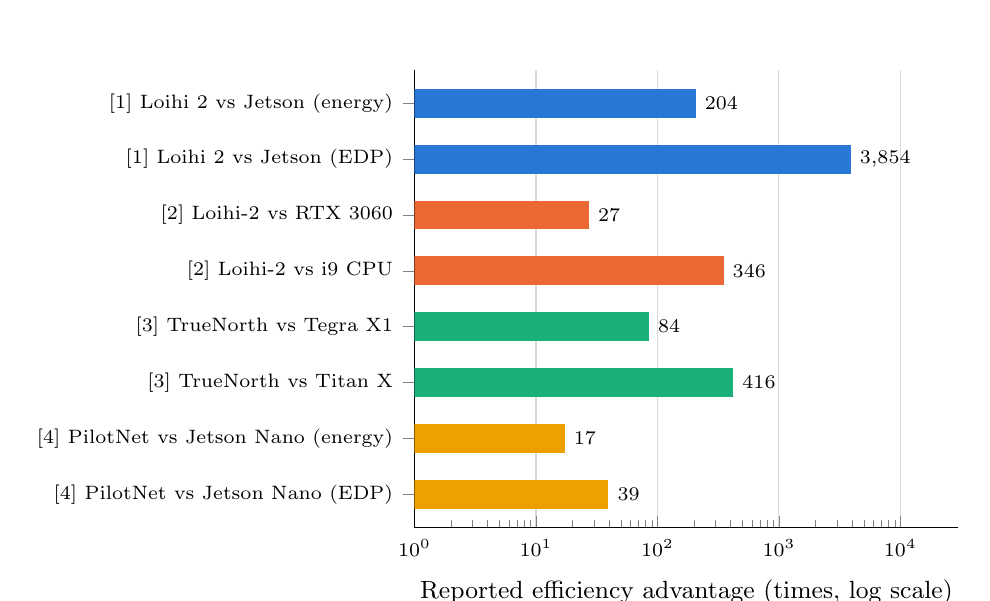
\begin{tikzpicture}
\begin{axis}[xbar, width=0.70\textwidth, height=7.4cm, bar width=10pt, xmode=log, xmin=1, xmax=30000, log origin=infty,
  ymin=0.4, ymax=8.6, ytick={1,...,8},
  yticklabels={{[4] PilotNet vs Jetson Nano (EDP)},{[4] PilotNet vs Jetson Nano (energy)},{[3] TrueNorth vs Titan X},{[3] TrueNorth vs Tegra X1},{[2] Loihi-2 vs i9 CPU},{[2] Loihi-2 vs RTX 3060},{[1] Loihi 2 vs Jetson (EDP)},{[1] Loihi 2 vs Jetson (energy)}},
  xlabel={Reported efficiency advantage (times, log scale)}, xmajorgrids, grid style={gridgray}, axis lines*=left,
  nodes near coords, nodes near coords align={horizontal}, point meta=rawx, nodes near coords style={font=\scriptsize, anchor=west, /pgf/number format/fixed, /pgf/number format/precision=0},
  y tick label style={font=\scriptsize}, tick label style={font=\scriptsize}, label style={font=\small}]
\addplot[fill=seriesA, draw=seriesA, bar shift=0pt] coordinates {(204,8) (3854,7)};
\addplot[fill=seriesB, draw=seriesB, bar shift=0pt] coordinates {(27,6) (346,5)};
\addplot[fill=seriesC, draw=seriesC, bar shift=0pt] coordinates {(84,4) (416,3)};
\addplot[fill=seriesD, draw=seriesD, bar shift=0pt] coordinates {(17,2) (39,1)};
\end{axis}
\end{tikzpicture}
\caption{Efficiency advantages over conventional hardware reported in the reviewed works, computed from their published tables: energy or EDP per inference for \cite{p1,p3,p4} (feedforward delay network at batch size 1 for \cite{p1}) and power efficiency in GOP/s/W for \cite{p2}}
\label{fig:cmp_gains}
\end{figure}

\section{Benchmarking Practices and Reproducibility}

\paragraph{} The works measure efficiency in different ways: \cite{p1} uses an IO-unconstrained mode on Loihi 2 and \texttt{jtop} power over several Jetson rails; \cite{p4} reports IO-bound and IO-free results and whole-SoC Jetson power; \cite{p3} scales TrueNorth's leakage to the cores used; and \cite{p2} does not describe its measurement method. Paper \cite{p4} shows how much this matters: Intel's PilotNet SDNN had similar energy but 65.4 ms latency in earlier measurements, against 2.50 ms with the newer software stack, because IO and system overheads had dominated. Fair evaluation therefore requires reporting accuracy alongside efficiency, separating IO from computation, stating which power rails are counted, and using well-tuned baselines at realistic batch sizes.

\section{Overall Comparative Insights}

\paragraph{} A consistent pattern emerges. \textbf{First}, neuromorphic hardware delivers order-of-magnitude gains in energy and EDP when network activity is sparse and computation is mapped to the chip's native primitives---delays \cite{p1}, crossbar cores \cite{p3}, or graded spikes \cite{p4}. \textbf{Second}, these gains are traded against accuracy, latency, or throughput in ways that depend on the coding scheme and on IO overheads. \textbf{Third}, ease of use is improving: conversion from standard PyTorch models \cite{p4} and export through NetX \cite{p1,p2} lower the barrier that TrueNorth's hand-built circuits \cite{p3} once represented. \textbf{Fourth}, evaluation practices are inconsistent, and system-level studies must report task accuracy and measurement details to be convincing. Hybrid pipelines that combine conventional training, hardware-aware conversion, and native temporal features such as delays are therefore the most promising path.

% ================= CHAPTER 5: APPLICATIONS =================
\chapter{Applications}

\section{Keyword Spotting and Voice Interfaces}

\paragraph{} Devices that listen continuously for wake words benefit directly: delay SNNs on Loihi 2 classify spoken digits in about 1.5 ms with under half a millijoule per sample \cite{p1}, suiting always-on voice control, acoustic event detection, and hearing aids.

\section{Autonomous Driving and Sensor Fusion}

\paragraph{} Vehicles fuse cameras, LIDAR, radar, GPS, and IMUs under tight power and latency budgets. Sub-millisecond sensor fusion at 1.5--2.5 W \cite{p2} and 40-fold lower EDP for PilotNet steering \cite{p4} suit always-on perception.

\section{Time-Series and Sequence Processing}

\paragraph{} Spike-based LSTMs at micro-joule energy \cite{p3} and delay networks \cite{p1} provide memory for physiological, industrial, and network streams, enabling anomaly detection and predictive maintenance.

\section{Drone Detection and Surveillance}

\paragraph{} Sky-watching sensors produce highly sparse video because only the targets move; a converted SDNN on Loihi 2 ran in real time at 112 FPS and 20 mJ per frame at a US Navy exercise \cite{p4}.

\section{Robotics and Edge IoT}

\paragraph{} Robots, drones, and IoT nodes paired with event cameras and tactile sensors can feed sparse data directly to neuromorphic units placed between sensors and actuators \cite{p2}, enabling low-power obstacle avoidance and gesture recognition.

% ================= CHAPTER 6: CHALLENGES AND FUTURE DIRECTIONS =================
\chapter{Challenges and Future Directions}

\paragraph{} Several obstacles remain before neuromorphic computing becomes a mainstream option for edge AI.

\section{Challenges Identified in the Reviewed Works}

\paragraph{} \textbf{Meszaros et al. \cite{p1}} are limited by the 62-step delay maximum, which costs about 5\% accuracy, and by single-seed, IO-unconstrained Loihi results. \textbf{Isik et al. \cite{p2}} report no task accuracy and use test data from an ideal environment. \textbf{Shrestha et al. \cite{p3}} need long phase lengths and hundreds of milliseconds per sample. \textbf{Brehove et al. \cite{p4}} gain little for dense, high-resolution video and face static power that grows with the number of chips.

\section{Cross-Cutting Challenges}

\paragraph{} The field faces \textbf{training complexity}, since direct SNN training is less mature than deep learning; \textbf{precision} losses from low-precision weights and spike coding; \textbf{IO overheads} that can dominate latency and energy \cite{p4}; \textbf{scalability} limits from inter-chip communication and static power; fragmented \textbf{tooling} and inconsistent \textbf{benchmarking}; and a \textbf{sensor mismatch}, as frame-based cameras do not produce sparse events.

\section{Future Research Directions}

\paragraph{} Promising directions are \textbf{event-based sensing} to supply naturally sparse inputs \cite{p4}; \textbf{richer temporal computation} with longer delays and adaptive neurons \cite{p1}; \textbf{hybrid training} that converts a conventional network and fine-tunes it with spike-aware methods; \textbf{real-time evaluation} on live sensor streams with reported accuracy \cite{p2}; \textbf{low-precision recurrent models} with short phase lengths \cite{p3}; and \textbf{standard benchmarks} and \textbf{on-chip learning} for fair comparison and adaptation in the field.

% ================= CHAPTER 7: CONCLUSION =================
\chapter{Conclusion}

\paragraph{} Conventional deep-learning hardware spends most of its energy moving data and recomputing unchanged inputs, which suits always-on edge applications poorly. Neuromorphic computing addresses this by computing with sparse spikes on chips that co-locate memory and processing. This seminar reviewed four works that train, convert, and deploy spiking neural networks on IBM's TrueNorth and Intel's Loihi 2.

\paragraph{} \textbf{Paper \cite{p1}}, the base paper, built a pipeline from EventProp delay learning to Loihi 2, raising feedforward keyword-spotting accuracy by up to 26.9 points and running up to 18 times faster with about 250 times less energy than a Jetson Orin Nano. \textbf{Paper \cite{p2}} applied Loihi-2 to sensor fusion on five driving datasets at 103.94 GOP/s/W with sub-millisecond inference. \textbf{Paper \cite{p3}} mapped an LSTM onto TrueNorth at 56 $\mu$J per sample. \textbf{Paper \cite{p4}} converted quantised PyTorch networks into sigma-delta networks, achieving 16 times lower energy and about 40 times lower EDP for PilotNet and a real-time field deployment. The comparison shows that \textbf{sparsity is the source of efficiency}, that \textbf{coding matters}, since few, information-rich spikes reduce latency and energy together, that \textbf{toolchains decide adoption}, and that \textbf{evaluation must be complete}, reporting accuracy and IO costs alongside efficiency.

\paragraph{} Across training strategy, coding, hardware constraints, and measured efficiency, a consistent pattern emerges: neuromorphic hardware delivers order-of-magnitude gains in energy and energy-delay product when network activity is sparse and computation uses the chip's native primitives, while accuracy, latency, and input-output overheads remain the main trade-offs. Pairing conventional deep-learning toolchains with hardware-aware conversion and event-based sensors is the most practical path to efficient deployment of spiking neural networks on Loihi 2 and TrueNorth.

% ================= REFERENCES =================
\begingroup
\setstretch{1.15}
\begin{thebibliography}{99}
\addcontentsline{toc}{chapter}{References}

\bibitem{p1}
B. Meszaros, J. C. Knight, J. Timcheck, and T. Nowotny, ``A complete pipeline for deploying SNNs with synaptic delays on Loihi 2,'' arXiv preprint arXiv:2510.13757, Oct. 2025.

\bibitem{p2}
M. Isik, K. Tiwari, M. B. Eryilmaz, and I. C. Dikmen, ``Accelerating sensor fusion in neuromorphic computing: A case study on Loihi-2,'' arXiv preprint arXiv:2408.16096, Aug. 2024.

\bibitem{p3}
A. Shrestha, K. Ahmed, Y. Wang, D. P. Widemann, A. T. Moody, B. C. Van Essen, and Q. Qiu, ``A spike-based long short-term memory on a neurosynaptic processor,'' in \textit{Proc. IEEE/ACM Int. Conf. Computer-Aided Design (ICCAD)}, 2017, pp. 631--637.

\bibitem{p4}
M. Brehove, S. A. Tumpa, E. Kyubwa, N. Menon, and V. Narayanan, ``Sigma-delta neural network conversion on Loihi 2,'' in \textit{Proc. Int. Conf. Neuromorphic Systems (ICONS '26)}, Chicago, IL, USA, Aug. 2026, arXiv:2505.06417.

\bibitem{merolla2014}
P. A. Merolla, J. V. Arthur, R. Alvarez-Icaza, A. S. Cassidy, J. Sawada, F. Akopyan, \textit{et al.}, ``A million spiking-neuron integrated circuit with a scalable communication network and interface,'' \textit{Science}, vol. 345, no. 6197, pp. 668--673, 2014.

\bibitem{davies2018}
M. Davies, N. Srinivasa, T.-H. Lin, G. Chinya, Y. Cao, S. H. Choday, \textit{et al.}, ``Loihi: A neuromorphic manycore processor with on-chip learning,'' \textit{IEEE Micro}, vol. 38, no. 1, pp. 82--99, 2018.

\bibitem{orchard2021}
G. Orchard, E. P. Frady, D. B. D. Rubin, S. Sanborn, S. B. Shrestha, F. T. Sommer, and M. Davies, ``Efficient neuromorphic signal processing with Loihi 2,'' in \textit{Proc. IEEE Workshop on Signal Processing Systems (SiPS)}, 2021, pp. 254--259.

\bibitem{oconnor2016}
P. O'Connor and M. Welling, ``Sigma delta quantized networks,'' arXiv preprint arXiv:1611.02024, 2016.

\bibitem{shrestha2018}
S. B. Shrestha and G. Orchard, ``SLAYER: Spike layer error reassignment in time,'' in \textit{Advances in Neural Information Processing Systems}, vol. 31, 2018.

\bibitem{wunderlich2021}
T. C. Wunderlich and C. Pehle, ``Event-based backpropagation can compute exact gradients for spiking neural networks,'' \textit{Scientific Reports}, vol. 11, no. 1, p. 12829, 2021.

\end{thebibliography}
\endgroup

\end{document}
